\part{{\scshape Conjuntos}}

\chapter{Os Axiomas e as Construções Essenciais}

\subsection*{Conjunto, Pertencimento e os Símbolos da Lógica Formal}

A noção de um \emph{conjunto} é uma noção primitiva na matemática. Intuitivamente, um conjunto é um objeto que tem \emph{elementos}. Cada elemento tem para com o conjunto em que está a relação de \emph{pertencimento}. Abstraindo mais essa noção, pensamos que todas as propriedades de um conjunto se resumem aos elementos que a ele pertencem, de modo que um conjunto é, de fato, seus elementos. A \emph{Teoria de Conjuntos} é uma teoria da lógica formal que procura formalizar essas ideias e estudar suas consequências. Neste livro, o tratamento da teoria de conjuntos será um tratamento informal, embora muita ênfase seja dada nos axiomas que constituem uma base para a teoria de conjuntos.

A lógica formal estuda sentenças formadas a partir de símbolos pré-determinados e fixos e as regras que dizem como essas sentenças se relacionam para formar novas sentenças. No tratamento formal da teoria de conjuntos, não há distinção entre conjunto e elemento. Ambos são somente denotados por letras de um alfabeto específico, e a relação de pertencimento é geralmente denotada pelo o símbolo $\in$. Se $X$ e $Y$ são conjuntos, a sentença ``o conjunto $X$ pertence ao conjunto $Y$'' ou ``o conjunto $X$ é elemento do conjunto $Y$'' é denotada por 
	\begin{equation*}
	X \in Y.
	\end{equation*}
Para afirmar que um conjunto $X$ não é elemento de um conjunto $Y$, ou seja, negar $X \in Y$, o símbolo usado é $\notin$ e se denota $X \notin Y$.

As teorias da lógica formal costumam ter axiomas, sentenças assumidas válidas a partir das quais deve-se inferir todas as outras sentenças da teoria. Axiomas, neste livro, serão enunciados, não como sentenças simbólicas, mas como sentenças em português. No entanto, alguns símbolos lógicos frequentemente facilitam e deixam mais claros os enunciados de sentenças na matemática. Os símbolos
	\begin{equation*}
	\forall \qquad \exists
	\end{equation*}
serão usados para substituirem as expressões ``para todo'' e ``existe'', respectivamente (desconsiderando possíveis flexões gramaticais). Eles indicam que alguma propriedade vale para todo elemento de um conjunto ou que existem elementos do conjunto para o qual a propriedade vale. O símbolo $\exists!$ significa que existe e é único e o símbolo $\nexists$ que não existe. Além desses, serão usados também os símbolos
	\begin{equation*}
	\entao \se \sse
	\end{equation*}
para significar a implicação material em cada sentido e a equivalência lógica. Por fim, para os conectivos `e' e `ou'  são usados os símbolos
	\begin{equation*}
	\e \qquad \ou
	\end{equation*}
Esse conectivos indicam, informalmente, que sentenças são ambas verdadeiras, no caso de `e', ou ao menos uma das duas é, no caso de `ou'. Os parênteses, que são comumente usados na lógica formal, serao substituidos por espaços, de modo que não haja ambiguidade. Mais detalhes sobre lógica formal e o uso dos símbolos lógicos serão suprimidos. Para aprofundamento em lógica e sistemas dedutivos, um livro indicado é \emph{Introduction to Logic}, de Alfred Tarski.

\section{Axiomas do Vazio, da Extensão e das Partes}

Os conceitos definidos nesta seção são \emph{igualdade} e \emph{contenção} de conjuntos. O primeiro axioma a ser considerado é o que define que existe um conjunto sem nenhum elemento, o \emph{conjunto vazio}. Esse conjunto tem um papel semelhante ao número zero. Ele é, de certo modo, um ``objeto neutro'' na teoria de conjuntos. Ao decorrer do desenvolvimento da teoria, essa frase sem significado matemática de fato ganhará um significado intuitivo e, em vários casos, uma definição mais precisa.

\begin{axi}[Vazio]
Existe o \emph{conjunto vazio}, um conjunto que não possui elementos. Denota-se esse conjunto por $\emptyset$.
\end{axi}

Formalmente, o axioma é $\exists x \forall y(y \notin x)$  e um conjunto vazio é um conjunto $x$ que satisfaz $\forall y(y \notin x)$. Como o conjunto vazio não possui elementos, sempre que se conclui que existe um elemento em $\emptyset$, ou seja, que existe $x \in \emptyset$, chega-se em uma contradição e a conclusão é que o que se assumiu para chegar na contradição é falso. Essa é uma forma padrão de se demonstrarem diversas proposições na lógica e na matemática.

O segundo axioma considerado é um axioma baseado em uma dos primeiras propriedades de um conjunto quando pensado intuitivamente: a ideia de que, quando abtrai-se da realidade, um conjunto é totalmente definido pelos elementos a que ele pertencem. Esse axioma se chama axioma da extensão e é a definição de \emph{igualdade} entre conjuntos.

\begin{axi}[Extensão]
Sejam $X$ e $Y$ conjuntos. Os conjuntos $X$ e $Y$ são \emph{iguais} se, e somente se, %todo elemento de $X$ pertence a $Y$ e todo elemento de $Y$ pertence a $X$.
	\begin{equation*}
	\forall x \in X \ x \in Y \e \forall y \in Y \ y \in X.
	\end{equation*}
Denota-se $X=Y$. Caso contrário, denota-se $X \neq Y$.
\end{axi}

Formalmente, o axioma é $\forall x \forall y (x = y \leftrightarrow \forall z (z \in x \leftrightarrow z \in y))$.  Quando se consideram conjuntos, é muito útil falar apenas de alguns de seus elementos, um conjunto desses elementos, possivelmente com alguma propriedade específica. Essa noção é a de um subconjunto, um conjunto cujos elementos pertencem todos a um outro conjunto considerado anteriormente. A definição de um subconjunto pode ser dada simplesmente a partir das noções primitivas já fornecidas, pois na ideia de subconjunto só são necessárias as noções de conunto e pertencimento, além dos símbolos lógicos.

\begin{defi}
Seja $X$ um conjunto. Um \emph{subconjunto} (ou uma \emph{parte}) de $X$ é um conjunto $Y$ que satisfaz
	\begin{equation*}
	\forall y \in Y \quad y \in X.
	\end{equation*}
Denota-se $Y \subseteq X$. Caso contrário, denota-se $Y \nsubseteq X$. Um subconjunto \emph{próprio} de $X$ é um subconjunto $Y \subseteq X$ tal que $Y \neq X$. Denota-se $Y \subset X$.
\end{defi}

Formalmente, a definição é $\forall x \forall y (x \subseteq y \leftrightarrow \forall z (z \in x \rightarrow z \in y))$. 

\begin{prop}
Seja $X$ um conjunto. Então
	\begin{enumerate}
	\item $\emptyset \subseteq X$;
	\item $X \subseteq \emptyset \entao X=\emptyset$.
	\end{enumerate}
\end{prop}
\begin{proof}
Suponha que $\emptyset$ não é subconjunto de $X$. Então existe $e \in \emptyset$ tal que $e \notin X$. Mas $e \in \emptyset$ é um absurdo, o que mostra que $\emptyset \subseteq X$.
\end{proof}

O próximo axioma considerado é o que garante que os subconjuntos de um conjunto dado formam um conjunto.

\begin{axi}[Partes]
Seja $X$ um conjunto. Então existe o \emph{conjunto das partes} de $X$, o conjunto que contém todos os subconjuntos de $X$. Denota-se $\p(X)$.
\end{axi}

\begin{prop}
Sejam $X$ e $Y$ conjuntos. Então
	\begin{equation*}
	X \subseteq Y \entao \p(X) \subseteq \p(Y).
	\end{equation*}
\end{prop}

\section{Axiomas da Especificação e do Par}

A noção intuitiva de subconjunto está diretamente relacionada à ideia de formar, a partir de um conjunto e uma propriedade, o subconjunto dos elementos que têm essa propriedade. A existência desse subconjunto é um axioma, chamado axioma da especificação porque a propriedade dada é um especificação dos elementos do conjunto original.

\begin{axi}[Especificação]
Sejam $X$ um conjunto e $\phi(x)$ uma sentença lógica. Existe o conjunto dos elementos de $X$ que satisfazem $\phi(x)$. Denota-se
	\begin{equation*}
	\set{x \in X}{\phi(x)}.
	\end{equation*}
\end{axi}

O próximo axioma garante, a partir da existência de dois, a existência de um novo conjunto cujos elementos são os dois conjuntos iniciais. Esse é o axioma do par. Embora a princípio sua necessidade não seja óbvia, esse axioma é importante --- ao menos útil --- para o desenvolvimento da teoria de conjuntos.

\begin{axi}[Par]
Sejam $X$ e $Y$ conjuntos. Existe o \emph{par} de $X$ e $Y$, o conjunto que tem como únicos elementos $X$ e $Y$. Denota-se $\{X,Y\}$.
\end{axi}

A partir do axioma do par pode-se formar o conjunto que tem como único elemento um  conjunto $X$ formando o par de $X$ e $X$. Esse conjunto é o conjunto unitário com único elemento $X$.

\begin{defi}
Seja $X$ um conjunto. O \emph{conjunto unitário} de elemento $X$ é o conjunto $\{X,X\}$. Denota-se $\{X\}$.
\end{defi}

\section{Axioma da União}

Nesta seção são apresentadas duas das contruções mais importantes da teoria de conjutos: a união e a interseção. A união de um conjunto de conjuntos denotado $C$ é o conjunto cujos elementos pertencem a algum conjunto que pertence $C$. O axioma da união afirma que esse conjunto existe.

\begin{axi}[União]
Seja $C$ um conjunto. Existe a \emph{união} de $C$, o conjunto dos elementos que pertencem a algum elemento de $C$. Denota-se $\bigcup C$. A união de um par $\{X,Y\}$ é denotada $X \cup Y$.
\end{axi}

Pode-se denotar a conjunto $\bigcup C$ por $\set{x}{\exists X \in C \quad x \in X}$.

\begin{prop} Sejam $X$ e $Y$ conjuntos. Então
	\begin{enumerate}
	\item $\bigcup \emptyset = \emptyset$;
	\item $X \subseteq Y \entao \bigcup X \subseteq \bigcup Y$.
	\end{enumerate}
\end{prop}
\begin{proof}
	\begin{enumerate}
	\item Suponha que $x \in \bigcup \emptyset$. Então $\exists X \in \emptyset$ tal que $x \in X$, o que é absurdo porque não pode existir $X \in \emptyset$.
	
	\item Seja $x \in \bigcup X$. Então existe $C \in X$ tal que $x \in C$. Como $X \subseteq Y$, segue que $C \in Y$, portanto $x \in \bigcup Y$.
	\end{enumerate}
\end{proof}

A interseção de um conjunto não vazio de conjuntos denotado $C$ é o conjunto cujos elementos pertencem a todos conjuntos que pertencem $C$. O conjunto interseção existe por consequêcia do axioma da especificação. Como $C$ é não vazio, basta considerar um conjunto $X \in C$ e a sentença lógica dada por
	\begin{equation*}
	\forall Y \in C \quad x \in Y.
	\end{equation*}
Desse modo, o conjunto interseção é $\set{x \in X}{\forall Y \in C \quad x \in Y}$.

\begin{defi}
Seja $C$ um conjunto não vazio. A \emph{interseção} de $C$ é o conjunto dos elementos que pertecem a todos elementos de $C$. Denota-se $\bigcap C$. A interseção de um par $\{X,Y\}$ é denotada $X \cap Y$.
\end{defi}

Pode-se denotar a conjunto $\bigcap C$ por $\set{x}{\forall X \in C \quad x \in X}$.

\begin{prop}
Seja $C$ um conjunto não vazio. Então
	\begin{equation*}
	\forall X \in C \qquad \bigcap C \subseteq X \subseteq \bigcup C.
	\end{equation*}
\end{prop}

\section{Axioma da Escolha}

Para que o axioma da escolha seja compreensível, deve-se definir alguns conceitos antes. Essencialmente, o axioma da escolha é sobre produto de conjuntos e sobre funções. O nome escolha, de fato, vem de uma função, a função escolha. Para definir o conceito de função, é necessário primeiro definir o que é um par ordenado de elementos de dois conjuntos e o que é o conjunto de pares ordenados desses conjunto, que é chamado produto dos conjuntos. A partir desse produto de dois conjuntos, definem-se função e, a partir de função, define-se o produto de qualquer conjunto.

\subsection*{Pares Ordenados, Produto de Par e Função}

\begin{defi}
Sejam $X$ e $Y$ conjuntos. O \emph{par ordenado} com \emph{primeira coordenada} $X$ e \emph{segunda coordenada} $Y$ é o conjunto
	\begin{equation*}
	(X,Y) := \{\{X\},\{X,Y\}\} \in \p\left(\p\left(X \cup Y\right)\right).
	\end{equation*}
\end{defi}

\begin{prop}
Sejam $X,Y,Z$ e $W$ conjuntos. Então
	\begin{equation*}
	(X,Y) = (Z,W) \sse X=Z \e Y=W.
	\end{equation*}
\end{prop}

\begin{defi}
Sejam $X$ e $Y$ conjuntos. O \emph{produto} de $X$ por $Y$ é o conjunto
	\begin{equation*}
	X \times Y := \set{(x,y) \in \p\left(\p\left(X \cup Y\right)\right)}{x \in X \e y \in Y}.
	\end{equation*}
\end{defi}

A existência desse conjunto depende da união de pares, do conjunto das partes e do axioma de especificação.

%\begin{defi}[Ênupla Ordenada]
%	Sejam $A$ e $B$ conjuntos. O \emph{par (ordenado)} dos elementos $a \in A$ e $b %\in B$ é o conjunto
%	\begin{equation*}
%	(a,b) := \{\{a\},\{a,b\}\}.
%	\end{equation*}
%De modo mais geral, sejam $A_1, \ldots, A_n$ $n$ conjuntos e $I := \{1,\ldots,n\}$. A \emph{n-upla (ordenada)} dos elementos $a_i \in A_i$, para todo $i \in I$, é definida indutivamente por
%	\begin{equation*}
%	(a_1,\ldots,a_n) := ((a_1,\ldots,a_{n-1}),a_n)	
%	\end{equation*}
%\end{defi}
%
%Assim, uma \emph{tripla} é
%	\begin{equation*}
%	(a,b,c) = ((a,b),c)=\{\{(a,b)\},\{(a,b),c\}\}=\{\{\{\{a\},\{a,b\}\}\},\{\{\{a\},\{a,b\}\},c\}\},
%	\end{equation*}
%claramente uma confusão desnecessária se não escrevermos $(a,b,c)$.

%\begin{prop}
%	Seja $A$ um conjunto não vazio. Então, para todos $a,b \in A$, vale $(a,b)=(b,a) \Leftrightarrow a=b$.
%\end{prop}
%\begin{proof}
%	Suponha $(a,b)=(b,a)$. Então $\{\{a\},b\}=\{\{b\},a\}$. Mas então $\{a\} \in (b,a)$, o que implica $\{a\}=\{b\}$ ou $\{a\}=a$. O primeiro caso implica $a=b$. O segundo caso é claramente impossível, pois nenhum conjunto pode ter como único elemento ele mesmo. A implicação contrária é trivial.
%\end{proof}
%
%\begin{prop}
%	Sejam $A_1,\ldots,A_n$ $n$ conjuntos não vazios. Então, para todos $a_i,b_i \in A_i$, $i \in \{1,\ldots,n\}$, vale
%	\begin{equation*}
%	(a_1,\ldots,a_n)=(b_1,\ldots,b_n) \Leftrightarrow a_i=b_i \quad \forall i \in \{1,\ldots,n\}.
%	\end{equation*}
%\end{prop}

\begin{defi}
Sejam $X$ e $Y$ conjuntos. Uma \emph{função} de $X$ para $Y$ é um conjunto $f \subseteq X \times Y$ que satisfaz
	\begin{equation*}
	\forall x \in X \ \exists! y \in Y \qquad (x,y) \in f.
	\end{equation*}
Esse $y$ é a \emph{imagem} de $x$, denotada por $f(x)$. Denotam-se $f: X \to Y$ e $f(x) := y$. Para qualquer conjunto $K \subseteq X$, defini-se a \emph{imagem} de $K$
	\begin{equation*}
	f(K)=\set{y \in Y}{\exists k \in K \quad y=f(k)},
	\end{equation*}
que é subconjunto de $Y$. Diz-se que o conjunto $f(X)$ é a \emph{imagem} de $f$.
\end{defi}

\begin{prop}
	Seja $f: A \to B$.
	\begin{enumerate}
	\item $A=\emptyset \sse f=\emptyset$.
	\item $B=\emptyset \entao A=\emptyset$.
	\end{enumerate}
\end{prop}
\begin{proof}
	\begin{enumerate}
	\item Suponhamos que $A=\emptyset$. Primeiro, notemos que $f=\emptyset$ é uma função de $\emptyset$ em $B$. Claramente, $f = \emptyset \subseteq \emptyset \times B$. Ainda, se $f$ não fosse função de $\emptyset$ em $B$, existiria $a \in \emptyset$ tal que não existe único $b \in B$ satisfazendo $(a,b) \in f$. Mas existir $a \in \emptyset$ é um absurdo. Logo $f$ é função. Por fim, se $g: \emptyset \times B$ é uma função, como $\emptyset \times B = \emptyset$, então $g \subseteq \emptyset \times B = \emptyset$, logo $g=\emptyset=f$.
	
	Reciprocamente, suponhamos $f=\emptyset$. Se $A \neq \emptyset$, seja $a \in A$. Como $f$ é função, existe $b \in B$ tal que $(a,b) \in f=\emptyset$, o que é absurdo. Portanto $A=\emptyset$.
	
	\item Suponhamos que $A \neq \emptyset$. Então existe $a \in A$ e, como $f$ é função, existe único $b \in \emptyset$ tal que $(a,b) \in f$. Mas $b \in \emptyset$ é absurdo, o que mostra que $A = \emptyset$.
	\end{enumerate}
\end{proof}

\subsection*{O Axioma da Escolha e Produto de Conjuntos}

\begin{defi}
Seja $C$ um conjunto. O \emph{produto} de $C$ é o conjunto
	\begin{equation*}
	\prod C := \set{f: C \to \bigcup C }{\forall X \in C \quad f(X) \in X}.
	\end{equation*}
	\begin{equation*}
	\prod C := \set{f \in \left(\bigcup C\right)^C }{\forall X \in C \quad f(X) \in X}.
	\end{equation*}
\end{defi}

\begin{prop}
Seja $C$ um conjunto. Então
	\begin{enumerate}
	\item $C = \emptyset \entao \prod C = \{\emptyset\}$;
	\item $\emptyset \in C \entao \prod C = \emptyset$.
	\end{enumerate}
\end{prop}
\begin{proof}
	\begin{enumerate}
	\item Como $C=\emptyset$, então $\bigcup \emptyset = \emptyset$. A função $\emptyset: \emptyset \to \emptyset$ é uma função em $\prod C$, pois satisfaz por vacuidade que $\forall X \in C \quad f(X) \in X$. Se não satisfizesse, existiria $X \in \emptyset$ tal que $f(X) \notin X$, o que é contradição. Isso mostra que $\emptyset \in \prod \emptyset$. Agora, seja $f \in \prod \emptyset$ função de $\emptyset$ em $\emptyset$. Como o domínio de $f$ é $\emptyset$, segue que $f=\emptyset$.
	
	\item Suponha que existe $f \in \prod C$. Então $f: C \to \bigcup C$ satisfaz que $\forall X \in C \quad f(X) \in X$. Como $\emptyset \in C$, existe $f(\emptyset) \in \bigcup C$ e, pela propriedade, $f(\emptyset) \in \emptyset$, contradição. Portanto $\prod C = \emptyset$.
	\end{enumerate}
\end{proof}

\begin{axi}[Escolha]
Seja $C$ um conjunto tal que $\emptyset \notin C$. Então $\prod C \neq \emptyset$.
\end{axi}



\section{Axiomas do Infinito e da Fundação}

\begin{defi}
Seja $X$ um conjunto. O \emph{sucessor} de $X$ é o conjunto
	\begin{equation*}
	X^+ := X \cup \{X\}.
	\end{equation*}
\end{defi}

\begin{axi}
Existe um \emph{conjunto indutivo}, um conjunto que contém $\emptyset$ e contém o sucessor de cada um de seus elementos.
\end{axi}

\begin{prop}
Seja $I$ um conjunto indutivo e $C$ o conjunto dos subconjuntos de $I$ que são indutivos. Então $\bigcap C$ é um conjunto indutivo.
\end{prop}

\section{Axioma da Substituição}

Os axiomas da especificação e do par são consequência do axioma da substituição.


\section*{Propriedades Gerais}

\subsection*{Contenção}

\begin{prop}
Sejam $X$, $Y$ e $Z$ conjuntos. Então
	\begin{enumerate}
	\item $X \subseteq X$;
	\item $X \subseteq Y \e Y \subseteq X \sse X=Y$;
	\item $X \subseteq Y \e Y \subseteq Z \entao X \subseteq Z$.
	\end{enumerate}
\end{prop}
\begin{proof}
	\begin{enumerate}
	\item Se $X=\emptyset$, então $\emptyset \subseteq X = \emptyset$. Logo $X \subseteq X$. Caso contrário, seja $x \in X$. Então $x \in X$. Logo $X \subseteq X$.
	\item $X \subseteq Y$ e $Y \subseteq X$ se, e somente se, $\forall x \in X \ x \in Y \e \forall y \in Y \ y \in X$, o que é equivalente a $X=Y$ pelo axioma da extensão.
	\item Se $X=\emptyset$, então $X \subseteq Z$. Caso contrário, seja $x \in X$. Então, como $X \subseteq Y$, $x \in Y$ e, como $Y \subseteq Z$, $x \in Z$. Logo $X \subseteq Z$.
	\end{enumerate}
\end{proof}

\subsection*{União e Interseção}

\begin{prop}
Sejam $X$, $Y$ e $Z$ conjuntos. Então
	\begin{enumerate}
	\item $X \cup \emptyset = X$;
	\item $X \cup Y = Y \cup X$;
	\item $(X \cup Y) \cup Z = X \cup (Y \cup Z)$;
	\item $X \cup X = X$;
	\item $X \subseteq Y \sse X \cup Y = Y$.
	\end{enumerate}
\end{prop}

\begin{prop}
Sejam $X,Y$ e $Z$ conjuntos. Então
	\begin{enumerate}
	\item $X \cap \emptyset = \emptyset$;
	\item $X \cap Y = Y \cap X$;
	\item $(X \cap Y) \cap Z = X \cap (Y \cap Z)$;
	\item $X \cap X = X$;
	\item $X \subseteq Y \sse X \cap Y = X$.
	\end{enumerate}
\end{prop}

\begin{prop}
Sejam $X$, $Y$ e $Z$ conjuntos. Então
	\begin{enumerate}
	\item $X \cap (Y \cup Z) = (X \cap Y) \cup (X \cap Z)$;
	\item $X \cup (Y \cap Z) = (X \cup Y) \cap (X \cup Z)$.
	\end{enumerate}
\end{prop}

\chapter{Famílias e Propriedades de Conjuntos}

\section{Famílias e Indexações}

Os axiomas já foram todos enunciados no capítulo anterior e as bases da teoria de conjuntos clássica está construída. Sendo assim, é necessário mudar a linguagem com que muitas das operações sobre conjuntos são tratadas, entre elas a união, a interseção e o produto. O conceito de uma família será definido nesta seção. Embora inicialmente a notação do capítulo anterior seja mais simples, eventualmente a notação de famílias com índices será necessária, por dois motivos principais. O primeiro é que esse conceito facilitará muito os enunciados de várias propriedades e teoremas na matemática eventualmente. O segundo é que tradicionalmente os matemáticos usam famílias e índices para denotar uniões, interseções, produtos e muitas outras noções. A ideia básica de uma família é a seguinte. Quando se define a união de um conjunto $C$ na teoria de conjuntos, a ideia intuitiva por trás da definição é que se estão unindo os conjuntos que são elementos de $C$. A união de um par $\{X,Y\}$ é denotada $X \cup Y$ não por acaso, essa notação indica um conjunto que está sendo formado com os elementos de $X$ e $Y$, não com os elementos dos elementos de $C$, como no caso de $\bigcup C$. 

Generalizando essa ideia, a união de três conjuntos $X_1,X_2,X_3$ pode ser denotada $X_1 \cup X_2 \cup X_3$ e o mesmo pode ser feito para qualquer quantidade finita de conjuntos. Mas para fazer o mesmo para uma quantidade qualquer de conjuntos, não é possível escrever esses conjuntos numa lista. Por isso surgiu a ideia de \emph{indexar} os conjuntos de $C$ que se pretende unir, usando a notação $(X_i)_{i \in I}$, sendo que cada $X_i$ é um elemento de $C$ e $i$ seu índice. Em seguida, indica-se na parte inferior do símbolo de união que os conjuntos indexados estão sendo unidos, de modo que $\bigcup C$ é denotado
	\begin{equation*}
	\bigcup_{i \in C} X_i.
	\end{equation*}

Essa notação tem a vantagem de estar mais próxima da intuição e também permite trabalhar com duplas uniões mais facilmente. As mesmas ideias são aplicadas para interseções e produtos. No entanto, ainda resta um problema, o problema principal. Tendo  já especificada qual é a notação que pretende-se aplicar, ainda falta definir o que é uma família somente a partir dos conceitos da teoria de conjuntos. Essa definição vem a seguir.

\begin{defi}
Sejam $C$ e $I$ conjuntos não vazios. Uma \emph{família} de elementos de $C$ indexados por $I$ é uma função $F: I \to C$. O conjunto $I$ é o \emph{conjunto de índices} da família. Denota-se isso por $(F_i)_{i \in I}$ e a imagem de $i \in I$ por $F$ é denotada $F_i$ e chamada de \emph{$i$-ésimo membro} da família.
\noindent
Uma \emph{sequência} é uma família em que $I=\N$, e uma \emph{sequência finita} é uma família em que $I \in \N$ (ou seja, $I=\{0,\ldots,n-1\}$ para algum $n \in \N$, e nesse caso diz-se $n$-sequência).
\end{defi}

Vale notar que uma família é vazia se, e somente se, $I=\emptyset$. Uma família é uma função e, portanto, quando se afirma que uma família, afirma-se que uma função é vazia, ou que é a função vazia. Mas isso ocorre se, e somente se, seu domínio, no caso o conjunto de índices, é vazio.

\begin{defi}
	Seja $X$ um conjunto não vazio. Uma \emph{indexação} de $X$ é uma família bijetiva $(x_i)_{i \in I}$ de elementos de $X$. Nesse caso, $X$ é um conjunto indexado por $I$ e denota-se $X=\{x_i\}_{i \in I}$.
\end{defi}

A noção de uma família é, de fato, mais motivada por notação do que por um conceito teórico, já que uma família é simplesmennte uma função sem nenhuma restrição, e a única diferença entre uma família é uma função é o contexto. Uma pergunta relevante, ainda, é se todo conjunto pode ser indexado por meio de uma família. Essa pergunta tem uma resposta óbvia e uma não óbvia, e ambas afirmam que sim. A resposta óbvia é que, para se indexar um conjunto $C$ basta considerar a função $F: C \to C$ definida para todo $X \in C$ por $F(X)=X$. Desse modo, essa é uma indexação do conjunto $X$. Mas essa resposta não satisfaz a tradição de indexar um quantidade finita de conjuntos $\{X,Y\}$ com números naturais. A resposta menos óbvia é que todo conjunto pode ser bem ordenado e, dessa forma, existe uma função de um número ordinal para o conjunto, logo uma indexação desse conjunto por um número ordinal. Os números naturais são os números ordinais finitos, o que significa que essa resposta menos óbvia condiz com a idexação que se faz usualmente de uma quantidade finita de conjuntos. Esse tópicos, no entanto, não serão abordados nesse capítulo.

\section{Propriedades de União e Interseção}

A partir da definição de família, pode-se definir a união e a interseção de uma família de conjuntos a partir da imagem do conjunto de índices $I$ pela função $C$, o conjunto $C(I) = \set{C_i}{i \in I}$. No entanto, um problema teórico se manifesta para se definir uma família de conjuntos. Se uma família é uma função de um conjunto de índices em um conjunto de elementos, para se definir uma família de conjuntos deveria existir um conjunto de todos conjuntos para fazer o papel de contradomínio de uma família. Esse conjunto, no entanto, não existe na teoria de conjuntos abordada neste livro, o que sugere que a definição de uma família de conjuntos depende, de fato, de um conjunto cujos elementos são os conjuntos da família de conjuntos. A existência desse conjunto de conjuntos é suposta, mas ele não é o conjunto de todos os conjuntos. Sendo assim, sempre que se enunciar uma família de conjuntos, essas ressalvas serão assumidas.

\begin{defi}
A \emph{união} de uma família $(C_i)_{i \in I}$ de conjuntos é o conjunto
\end{defi}
	\begin{equation*}
	\bigcup_{i \in I} C_i := \bigcup C(I).
	\end{equation*}
A \emph{interseção} de uma família não vazia $(C_i)_{i \in I}$ de conjuntos é o conjunto
	\begin{equation*}
	\bigcap_{i \in I} C_i := \bigcap C(I).
	\end{equation*}
\noindent
Quando $I$ for finito, pode-se denotar
	\begin{equation*}
	C_1 \cup \cdots \cup C_n := \bigcup_{i \in I} C_i \qquad \e \qquad C_1 \cap \cdots \cap C_n := \bigcap_{i \in I} C_i.
	\end{equation*}
	
\begin{prop}
	Seja $(C_i)_{i \in I}$ uma família de conjuntos. Então
	\begin{enumerate}
	\item $\forall i \in I \quad C_i = \emptyset \qquad \Leftrightarrow \qquad \displaystyle \bigcup_{i \in I} C_i = \emptyset$.
	
	\item $\displaystyle \exists i \in I \quad C_i = \emptyset \qquad \Rightarrow \qquad \bigcap_{i \in I} C_i = \emptyset$.
	\end{enumerate}
\end{prop}

\begin{prop}
Sejam $X$ um conjunto e $(C_i)_{i \in I}$ uma família não vazia de subconjuntos de $X$. Então
	\begin{enumerate}
	\item $\displaystyle \left( \bigcap_{i \in I} C_i \right)^\complement = \bigcup_{i \in I} (C_i)^\complement$
	
	\item $\displaystyle \left( \bigcup_{i \in I} C_i \right)^\complement = \bigcap_{i \in I} (C_i)^\complement$
	\end{enumerate}
\end{prop}
\begin{proof}
	\begin{enumerate}
	\item Para isso, basta notar que $c \in \left( \bigcap_{i \in I} C_i \right)^\complement$ se, e somente se, $c \notin \bigcap_{i \in I} C_i$. Mas isso ocorre se, e somente se, existe $i \in I$ tal que $c \notin C_i$. Essa afirmação é equivalente a $c \in (C_i)^\complement$ que, por sua vez, é equivalente a $ c \in \bigcup_{i \in I} (C_i)^\complement$.
	
		\item Como, para todo conjunto $C$, $(C^\complement)^\complement = C$, segue do item anterior que
		\begin{equation*}
		\displaystyle \left( \bigcup_{i \in I} C_i \right)^\complement = \left( \bigcup_{i \in I} ((C_i)^\complement)^\complement \right)^\complement = \left( \left( \bigcap_{i \in I} (C_i)^\complement \right)^\complement \right)^\complement = \bigcap_{i \in I} (C_i)^\complement.
		\end{equation*}
	\end{enumerate}
\end{proof}

\begin{prop}
Seja $(C_{ij})$ uma família não vazia de conjuntos. Então
	\begin{equation*}
	\bigcup_{i \in I} \left( \bigcap_{j \in J} C_{ij} \right) \subseteq \bigcap_{j \in J} \left( \bigcup_{i \in I} C_{ij} \right)
	\end{equation*}
\end{prop}

\begin{prop}
Seja $(C_{ij})$ uma família não vazia de conjuntos. Então
	\begin{enumerate}
	\item $\displaystyle\bigcap_{i \in I} \p\left(C_i \right) = \p\left(\displaystyle\bigcap_{i \in I} C_i \right)$;
	\item $\displaystyle\bigcup_{i \in I} \p\left(C_i \right) \subseteq \p\left(\displaystyle\bigcup_{i \in I} C_i \right)$.
	\end{enumerate}
\end{prop}

\cleardoublepage
\section{Produto de Conjuntos}

   \begin{defi}
Seja $(C_i)_{i \in I}$ uma família de conjuntos. O \emph{produto} de $(C_i)_{i \in I}$ é o conjunto
	\begin{equation*}
	\prod_{i \in I} C_i := \set{(c_i)_{i \in I}}{\forall i \in I \quad c_i \in C_i}.
	\end{equation*}
As famílias $(c_i)_{i \in I}$ são de elementos em $\bigcup_{i \in I} C_i$.
\end{defi}

\begin{defi}
Seja $(C_i)_{i \in I}$ uma família de conjuntos e $i \in I$. A \emph{projeção canônica} de $\prod_{i \in I} C_i$ em $C_i$ é a função
	\begin{align*}
	\func{\pi_i}{\prod_{i \in I} C_i}{C_i}{(c_i)_{i \in I}}{c_i}.
	\end{align*}
\end{defi}

\begin{prop}[Propriedade Universal]
Sejam $(C_i)_{i \in I}$ uma família de conjuntos, $X$ um conjunto e, para todo $i \in I$, $f_i: X \to C_i$ uma função. Então existe uma única função $f: X \to \prod_{i \in I} C_i$ tal que, para todo $i \in I$, $\pi_i \circ f = f_i$ (o diagrama comuta).
\begin{figure}
\centering
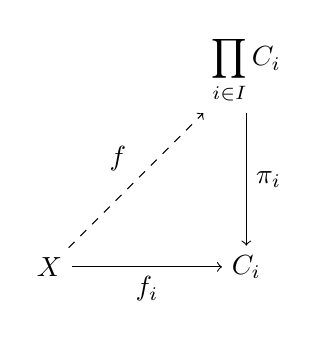
\begin{tikzpicture}[node distance=2.5cm, auto]
	\node (P) {$\displaystyle\prod_{i \in I} C_i$};
	\node (Ci) [below of=P] {$C_i$};
	\node (X) [left of=Ci] {$X$};
	\draw[->] (X) to node [swap] {$f_i$} (Ci);
	\draw[->, dashed] (X) to node {$f$} (P);
	\draw[->] (P) to node {$\pi_i$} (Ci);
\end{tikzpicture}
\end{figure}
\end{prop}
\begin{proof}
Defina a função
	\begin{align*}
	\func{f}{X}{\prod_{i \in I} C_i}{x}{(f_i(x))_{i \in I}}.
	\end{align*}
Para todo $x \in X$ e para todo $i \in I$,
	\begin{equation*}
	\pi_i \circ f(x) = \pi_i (f(x)) = \pi_i ((f_i(x))_{i \in I}) = f_i(x).
	\end{equation*}
Portanto $\pi_i \circ f = f_i$. Isso mostra a existência da $f$. Para a unicidade, seja $\overline{f}: X \to \prod_{i \in I} C_i$ função tal que, para todo $i \in I$, $\pi_i \circ \overline{f} = f_i$. Seja $x \in X$.  Como $\overline{f}(x) \in \prod_{i \in I} C_i$, $\overline{f}(x) = (x_i)_{i \in I}$. Da propriedade comutativa de $\overline{f}$, segue que, para todo $i \in I$,
	\begin{equation*}
	x_i = \pi_i \circ \overline{f}(x) = f_i(x).
	\end{equation*}
Como $f(x) = (f_i(x))_{i \in I}$, isso mostra que $\overline{f}(x) = f(x)$. Portanto $\overline{f} = f$.
\end{proof}



%O axioma da escolha reescrito para famílias é o seguinte. Para toda família não vazia $(C_i)_{i \in I}$ de conjuntos (disjuntos) não vazios, existe uma função (\emph{função escolha}) $E: I \to \bigcup_{i \in I} C_i$ tal que, para todo $i \in I$, $E(i) \in C_i$.

%\begin{prop}
%	Seja $(C_i)_{i \in I}$ uma família não vazia de conjuntos. Então
%	\begin{equation*}
%	\prod_{i \in I} C_i = \emptyset \qquad \Leftrightarrow \qquad \exists i \in I \quad C_i = \emptyset.
%	\end{equation*}
%\end{prop}
%\begin{proof}
%	Primeiro, suponhamos que $(C_i)_{i \in I}$ é uma família de conjuntos não vazios. Então, pelo axioma da escolha, existe uma função $E: I \to \bigcup_{i \in I} C_i$ tal que, para todo $i \in I$, $E(i) \in C_i$. Assim, $E \in \prod_{i \in I} C_i$, o que mostra que $\prod_{i \in I} C_i \neq \emptyset$. Reciprocamente, suponhamos que existe alguma $i \in I$ tal que $C_i = \emptyset$. Então, se existisse $c \in \prod_{i \in I} C_i$, seguiria que $c(i) \in C_i = \emptyset$, o que é absurdo. Logo $\prod_{i \in I} C_i = \emptyset$.
%\end{proof}





\section{Coproduto de Conjuntos}

\begin{defi}
Seja $(C_i)_{i \in I}$ uma família não vazia de conjuntos. O \emph{coproduto} de $(C_i)_{i \in I}$ é o conjunto
	\begin{equation*}
	\coprod_{i \in I} C_i :=\set{(i,c)}{i \in I \e c \in C_i}.
	\end{equation*}
\end{defi}

\begin{defi}
Seja $(C_i)_{i \in I}$ uma família de conjuntos e $i \in I$. A \emph{inclusão canônica} de $C_i$ em $\coprod_{i \in I} C_i$ é a função
	\begin{align*}
	\func{\iota_i}{C_i}{\coprod_{i \in I} C_i}{c}{(i,c)}.
	\end{align*}
\end{defi}

\begin{prop}[Propriedade Universal]
Sejam $(C_i)_{i \in I}$ uma família de conjuntos, $X$ um conjunto e, para todo $i \in I$, $f_i: C_i \to X$ uma função. Então existe uma única função $f: \coprod_{i \in I} C_i \to X$ tal que, para todo $i \in I$, $f \circ \iota_i = f_i$ (o diagrama comuta).
\begin{figure}
\centering
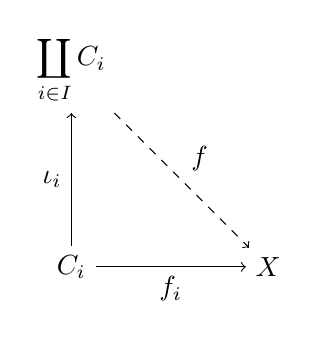
\begin{tikzpicture}[node distance=2.5cm, auto]
	\node (Ci) {$C_i$};
	\node (S) [above of=Ci] {$\displaystyle\coprod_{i \in I} C_i$};
	\node (X) [right of=Ci] {$X$};
	\draw[->] (Ci) to node [swap] {$f_i$} (X);
	\draw[->, dashed] (S) to node {$f$} (X);
	\draw[->] (Ci) to node {$\iota_i$} (S);
\end{tikzpicture}
\end{figure}
\end{prop}
\begin{proof}
Defina a função
	\begin{align*}
	\func{f}{\coprod_{i \in I} C_i}{X}{(i,c)}{f_i(c)}.
	\end{align*}
Seja $i \in I$ e $c \in C_i$. Então
	\begin{equation*}
	f \circ \iota_i(c) = f(\iota_i(c)) = f(i,c) = f_i(c).
	\end{equation*}
Portanto $f \circ \iota_i = f_i$. Isso mostra a existência da $f$. Para a unicidade, seja $\overline{f}: \coprod_{i \in I} C_i \to X$ função tal que, para todo $i \in I$, $\overline{f} \circ \iota_i = f_i$. Seja $x \in \coprod_{i \in I} C_i$. Existem $i \in I$ e $c \in C_i$ tais que $x=(i,c)$. Da propriedade comutativa de $\overline{f}$, segue que
	\begin{equation*}
	\overline{f}(x) = \overline{f}(i,c) = \overline{f}(\iota_i(x)) = \overline{f} \circ \iota_i(c) = f_i(c) = f(i,c) = f(x).
	\end{equation*}
Isso mostra que $\overline{f}=f$.
\end{proof}


%\cleardoublepage
%\begin{figure}
%\centering
%\begin{tikzpicture}[node distance=4cm, auto]
%	\node (P) {$\displaystyle\prod_{i \in I} C_i$};
%	\node (Ci) [below of=P] {$C_i$};
%	\node (X) [left of=Ci] {$X$};
%	\node (S) [below of=Ci] {$\displaystyle\coprod_{i \in I} C_i$};
%	\node (Y) [right of=Ci] {$Y$};	
%	\draw[->] (X) to node [swap] {$f_i$} (Ci);
%	\draw[->, dashed] (X) to node {$f$} (P);
%	\draw[->] (P) to node {$\pi_i$} (Ci);
%	\draw[->] (Ci) to node {$g_i$} (Y);
%	\draw[->, dashed] (S) to node [swap] {$g$} (Y);
%	\draw[->] (Ci) to node [swap] {$\iota_i$} (S);
%\end{tikzpicture}
%\caption*{Os diagramas comutativos do \\produto e do coproduto de conjuntos.}
%\end{figure}





\cleardoublepage
\subsection{Propriedades de Produto e Coproduto}

\begin{prop}
	Seja $(C_{ij})_{(i,j) \in I \times J}$ uma família de conjuntos. Então
	\begin{enumerate}
	\item $\displaystyle \bigcup_{j \in J} \left(\prod_{i \in I} C_{ij}\right) \subseteq \prod_{i \in I} \left(\bigcup_{j \in J} C_{ij}\right)$;
	\item $\displaystyle \bigcap_{j \in J} \left(\prod_{i \in I} C_{ij}\right) = \prod_{i \in I} \left(\bigcap_{j \in J} C_{ij}\right)$.
	\end{enumerate}
\end{prop}
\begin{proof}
	\begin{enumerate}	
	\item \begin{align*}
	\displaystyle c \in  \bigcup_{j \in J} \left(\prod_{i \in I} C_{ij}\right)
		& \entao \exists j \in J \left(c \in \prod_{i \in I} C_{ij} \right) \\
		& \entao \exists j \in J \ \forall i \in I \left(c_i \in C_{ij} \right) \\
		& \entao \forall i \in I \left(c \in \bigcup_{j \in J} C_{ij} \right) \\
		& \entao  c \in \prod_{i \in I} \left(\bigcup_{j \in J} C_{ij}\right).
	\end{align*}
	
	\item 	
	\begin{align*}
	c \in \displaystyle \bigcap_{j \in J} \left(\prod_{i \in I} C_{ij}\right)
		& \sse \forall j \in J \left(c \in \prod_{i \in I} C_{ij} \right) \\
		& \sse \forall j \in J \ \forall i \in I \left(c_i \in C_{ij} \right) \\
		& \sse \forall i \in I \ \forall j \in J \left(c_i \in C_{ij} \right) \\
		& \sse \forall i \in I \left(c_i \in \bigcup_{j \in J} C_{ij} \right) \\
		& \sse  c \in \prod_{i \in I} \left(\bigcap_{j \in J} C_{ij}\right).
	\end{align*}
	\end{enumerate}
\end{proof}

Notemos que a inclusão contrária no primeiro item nao vale. Suponhamos que para um $j_0 \in J$, todos os $C_{ij_0}$ são vazios, mas para todos outros $j \in J$, os $C_{ij}$ não são vazios. Então o produto desses $C_{ij}$ será sempre vazio, pois sempre tem um dos elementos do produto vazio, e então a união desses produtos será vazia; no entanto, a união desses $C_{ij}$ não será nenhuma vazia e, então, o produto não seráa vazio (pelo axioma da escolha).

\begin{prop}
\label{conj:prop.im.inv.prod}
Sejam $X$ um conjunto, $(Y_i)_{i \in I}$ uma família de conjuntos, $(S_i)_{i \in I}$ uma família de subconjutos de $(Y_i)_{i \in I}$, $f: X \to \prod_{i \in I} Y_i$ uma função e, para todo $i \in I$, $f_i := \pi_i \circ f$. Então
	\begin{equation*}
	f\inv\left( \prod_{i \in I} {S_i} \right) = \bigcap_{i \in I} f_i\inv (S_i).
	\end{equation*}
\end{prop}
\begin{proof}
Note que $x \in f\inv(\prod_{i \in I} {S_i})$ é equivalente a $f(x) \in \prod_{i \in I} {S_i}$, que por sua vez ocorre se, e somente se, para todo $i \in I$, $\pi_i(f(x)) \in S_i$. Como $f_i(x)=\pi_i(f(x)) \in S_i$, isso é equivalente a, para todo $i \in I$, $x \in f_i\inv (S_i)$.
\end{proof}





%\begin{defi}
%Seja $C$ um conjunto não vazio. A \emph{soma} de $C$ é o conjunto
%	\begin{equation*}
%	\coprod C := \set{(X,x) \in C \times \bigcup C}{x \in X}.
%	\end{equation*}
%\end{defi}

%Vale notar que a soma de $C$ existe porque é um subconjunto de $\p\left(C \times \bigcup C \right)$, logo é um conjunto pelo axioma da especificação.

%Definimos a seguir uma nova operação em uma família $(C_i)_{i \in I}$, a soma, também chamada de união disjunta. Em vez de unirmos todos elementos de $(C_i)_{i \in I}$, indexamos cada um deles com o índice do conjunto da família a que ele pertence para que, se um mesmo elemento, digamos $c$, pertencer $C_{i_1}$ e $C_{i_2}$, $i_1,i_2 \in I$ distintos, então na união disjunta $(c,i_1)$ e $(c,i_2)$ serão elementos distintos, enquanto que na união não haverá distinção.



%\begin{conj}
%	Seja $(C_i)_{i \in I}$ uma família não vazia de conjuntos. Então
%	\begin{equation*}
%	\coprod_{i \in I} C_i = \emptyset \qquad \Leftrightarrow \qquad \forall i \in I \quad C_i = \emptyset.
%	\end{equation*}
%\end{conj}


\subsubsection*{Notação alternativa}

\begin{equation*}
\prod_{i \in I} C_i = \set{\lceil c_i \rceil_{i \in I}}{\forall i \in I \; c_i \in C_i}
\end{equation*}

$\lceil c_i \rceil_{i \in I} = c: I \to \bigcup_{i \in I} C_i$

\begin{equation*}
\coprod_{i \in I} C_i = \set{\lfloor c \rfloor_i}{i \in I, c \in C_i}
\end{equation*}

$\lfloor c \rfloor_i = (i,c)$




\section{Complementares e Diferença Simétrica}

\begin{defi}
Sejam $X$ e $Y$ conjuntos. O \emph{complementar relativo} de $Y$ em $X$ é o conjunto
	\begin{equation*}
	X \setminus Y := \set{x \in X}{x \notin Y}.
	\end{equation*}
\end{defi}

\begin{defi}
Sejam $X$ um conjunto e $S$ um subconjunto de $X$. O \emph{complementar} de $S$ em $X$ é o conjunto
	\begin{equation*}
	S^\complement := X \setminus S.
	\end{equation*}
%Seja $\mathcal A \subseteq \p(A)$. O \emph{conjunto complementar} de $\mathcal A$ em $A$ é o conjunto
%	\begin{equation*}
%	\complementlement(\mathcal A) := \{X^\complement : X \in \mathcal A\}.
%	\end{equation*}
\end{defi}

\begin{defi}
Sejam $X$ e $Y$ conjuntos. A \emph{diferença simétrica} de $X$ e $Y$ é o conjunto
	\begin{equation*}
	X \difsim Y := (X \setminus Y) \cup (Y \setminus X).
	\end{equation*}
\end{defi}

\subsection{Propriedades}

\begin{prop}
Sejam $X$, $Y$ subconjuntos de $U$. Então
	\begin{enumerate}
	\item $(X^\complement)^\complement = X$;
	\item $\emptyset^\complement = U$ e $U^\complement = \emptyset$;
	\item $X \cap X^\complement = \emptyset$ e $X \cup X^\complement = U$;
	\item $X \subseteq Y \sse Y^\complement \subseteq X^\complement$.
	\item $(X \cup Y)^\complement = X^\complement \cap Y^\complement$ e $(X \cap Y)^\complement = X^\complement \cup Y^\complement$.
	\end{enumerate}
\end{prop}




\section{Coberturas e Partições}

\begin{defi}
Seja $X$ um conjunto. Uma \emph{cobertura} de $X$ é uma família $(C_i)_{i \in I}$ de subconjuntos de $X$ cuja união é $X$:
	\begin{equation*}
	\bigcup_{i \in I} C_i = X.
	\end{equation*}
Um \emph{subcobertura} de uma cobertura $(C_i)_{i \in I}$ de $X$ é uma cobertura $(C_i)_{i \in J}$ de $X$, com $J \subseteq I$.
\end{defi}

\begin{defi}
Seja $X$ um conjunto. Uma \emph{partição} de $X$ é um conjunto $\mathcal P \subseteq \p(X)$ de subconjuntos de $X$ que satisfaz
	\begin{enumerate}
	\item $\emptyset \notin \mathcal P$;
	\item $\displaystyle\bigcup \mathcal P = X$;
	\item Para todos conjuntos distintos $C_0,C_1 \in \mathcal P$, $C_0 \cap C_1 = \emptyset$.
	\end{enumerate}
Os conjuntos $C \in \mathcal P$ são as \emph{células} de $\mathcal P$.
\end{defi}

Uma partição, se identidicamos um subconjunto de $\p(X)$ com uma família de sunconjuntos de $X$, é uma cobertura de $X$ por conjuntos disjuntos (logo distintos) que não contém o conjunto vazio.

\subsection{Refinamento de Partições}

\begin{defi}
Sejam $X$ um conjunto e $\mathcal P$ uma partição de $X$. Um \emph{refinamento} (\emph{superpartição}) de $\mathcal P$ é uma partição $\mathcal R$ de $X$ que satisfaz: para toda célula $D \in \mathcal R$, existe uma célula $C \in \mathcal P$ tal que $D \subseteq C$. Denota-se $\mathcal P \leq \mathcal R$. Diz que $\mathcal P$ é um \emph{engrossamento} (\emph{subpartição}) de $\mathcal R$.
\end{defi}

\begin{prop}
Sejam $X$ um conjunto e $\mathcal P,\mathcal R$ partições de $X$ tais que $\mathcal P \leq \mathcal R$. Então
	\begin{enumerate}
	\item $\card{\mathcal P} \leq \card{\mathcal R}$;
	\item Para cada célula $C \in \mathcal P$, o conjunto
		\begin{equation*}
		\mathcal R|_C := \set{D \in \mathcal R}{D \subseteq C}
		\end{equation*}
é uma partição de $C$.
	\end{enumerate}
\end{prop}
\begin{proof}
	\begin{enumerate}
	\item Por definição de refinamento, para toda célula $D \in \mathcal R$ existe célula $C \in \mathcal P$ tal que $D \subseteq C$. Notemos que essa célula $C$ é única pois, se existir célula $C' \in \mathcal P$ tal que $D \subseteq C'$, então $D \subseteq C \cap C'$ e, como $D \neq \emptyset$, segue que $C =C'$. Assim, consideramos a função que mapeia, para cada célula $D \in \mathcal R$ a célula $C_D \in \mathcal P$ tal que $D \subseteq C_D$:
	\begin{align*}
	\func{f}{\mathcal R}{\mathcal P}{D}{C_D}.
	\end{align*}
Mostremos que essa função é sobrejetiva. Para isso, seja $C \in \mathcal P$. Como $\bigcup \mathcal R = X$, para todo $x \in C \subseteq X$ existe $D \in \mathcal R$ tal que $x \in D$. Como $C \neq \emptyset$, existe $x \in C$, logo existe $D \in \mathcal R$ tal que $x \in D$. Por definição de refinamento, existe $C' \in \mathcal P$ tal que $D \subseteq C'$, o que implica $x \in C'$. Como $x \in C' \cap C$, segue que $C=C'$, e concluímos que $D \subseteq C$. Isso mostra que $f(D)=C$, logo que $f$ é sobrejetiva. Concluímos, então, que $\card{\mathcal P} \leq \card{\mathcal R}$.
	
	\item As propriedades 1 e 3 são evidentes por que $\mathcal R$ é partição. Para a propriedade 2, seja $C \in \mathcal P$ e $U := \bigcup \set{D \in \mathcal R}{D \subseteq C}$. Notemos que $C=U$. Para mostrar isso, seja $x \in C$. Então existe $D \in \mathcal R$ tal que $x \in D$, pois $\bigcup \mathcal P=X$. Por definição de refinamento, existe $C' \in \mathcal P$ tal que $D \subseteq C'$, portanto $x \in C'$. Como $x \in C' \cap C$, segue que $C=C'$. concluímos que $D \subseteq C$, portanto que $x \in U$, o que mostra $C \subseteq U$. Reciprocamente, para todo $D \in U$, $D \subseteq C$, portanto $U \subseteq C$, e concluímos que $C=U$.
	\end{enumerate}
\end{proof}

\begin{prop}
Sejam $X$ um conjunto. A relação de refinamento $\leq$ no conjunto de partições de $X$ é uma relação de ordem parcial.
\end{prop}

\begin{defi}
Sejam $X$ um conjunto e $(\mathcal P_i)_{i \in I}$ uma família de partições de $X$. O \emph{refinamento comum} a $(\mathcal P_i)_{i \in I}$ é o conjunto
	\begin{equation*}
	\bigvee_{i \in I} \mathcal P_i := \set{\bigcap_{i \in I} C_i}{i \in I,\  C_i \in \mathcal P_i \e \bigcap_{i \in I} C_i \neq \emptyset}.
	\end{equation*}
\end{defi}

\begin{prop}
Sejam $X$ um conjunto e $(\mathcal P_i){i \in I}$ uma família de partições de $X$. O refinamento comum $\bigvee_{i \in I} \mathcal P_i$ a $(\mathcal P_i)_{i \in I}$ é a menor partição de que $X$ que refina $\mathcal P_i$ para todo $i \in I$.
\end{prop}
\begin{proof}
Primeiro, mostremos que $\mathcal P := \bigvee_{i \in I} \mathcal P_i$ é uma partição. Por definição, $\emptyset \notin \mathcal P$. Seja $x \in X$. Então, para cada $i \in I$, existe $C_i \in \mathcal P_i$ tal que $x \in C_i$, pois $\bigcup \mathcal P_i = X$. Sendo assim, $x \in \bigcap_{i \in I} C_i$, portanto $X \subseteq \bigcup \mathcal P$, e segue que $\bigcup \mathcal P = X$. Por fim, sejam $C=\bigcap_{i \in I} C_i, D=\bigcap_{i \in I} D_i \in \mathcal P$. Se $C \neq D$, então existe $x \in C\setminus D$ ou existe $x \in D \setminus C$. Sem perda de generalidade, suponha o primeiro. Então, existe $i \in I$ tal que $x \notin D_i$. Como $x \in C$, então $x \in C_i$, portanto $C_i \neq D_i$. Mas então, como $\mathcal P_i$ é partição, $C_i \cap D_i = \emptyset$. Por fim, como $C \subseteq C_i$ e $D \subseteq D_i$, segue que $C \cap D = \emptyset$.

Agora mostraremos que $\mathcal P$ é refinamento de $\mathcal P_i$ para todo $i \in I$. Sejam $i \in I$ e $C \in \mathcal P$. Então $\mathcal P=\bigcap_{i \in I} C_i$, portanto $C_i \in \mathcal P_i$. Por fim, sejam $\mathcal R$ partição de $X$ que é refina $\mathcal P_i$ para todo $i \in I$ e $D \in \mathcal R$ uma célula. Então, para todo $i \in I$, existe $C_i \in \mathcal P_i$ tal que $D \subseteq C_i$. Portanto $D \subseteq \bigcap_{i \in I} C_i$, e como $\bigcap_{i \in I} C_i \in \mathcal P$, segue que $\mathcal P \leq \mathcal R$.
\end{proof}

Alguns tipos especiais de partições são úteis na teoria de intergação de Riemmann. Em $\R^1$, essas partições são chamadas de partições de intervalo, e são representadas como um número finito de pontos em um intervalo. Quando generaliza-se para dimensões maiores, usam-se $n$-retângulos, que são conjuntos em $\R^n$ produtos de $n$ intervalos limitados. Podemos fixar um critério a mais, o de que um $n$-retângulo é produto de intervalos fechados em baixo e abertos em cima. Nesse caso, podemos definir que uma partição cujos elementos são $n$-retângulos é uma \emph{malha}.

Alternativamente, quando temos uma medida, que é o caso de $\R^n$, podemos enfraquecer a restrição de que as células de uma partição são iguais ou disjuntas para a de que são iguais ou \emph{quase disjuntas} \--- a interseção tem medida zero \--- e a restrição de que cobrem para a restrição de que a união da partição é quase total \--- seu complementar tem medida nula \--- e por fim, de que nenhum elemento da partição é quase vazio \--- tem medida nula \--- e definir que isso é uma $\mu$-partição ou \emph{quase partição com respeito a $\mu$}.



























\chapter{Funções}

\begin{defi}
Sejam $X$ e $Y$ conjuntos. Uma \emph{relação} $R$ de $X$ para $Y$ é um subconjunto de $X \times Y$. Os conjuntos $X$ e $Y$ são, respectivamente, o \emph{domínio} e o \emph{contradomínio} de $R$. Denota-se $x \mathrel{R} y$ para $(x,y) \in R$.
\end{defi}

\begin{defi}
Seja $R$ uma relação de $X$ em $Y$. A \emph{relação inversa} de $R$ é a relação $R\inv$ de $Y$ em $X$ definida por
	\begin{equation*}
	\forall x \in X\ \forall y \in Y \qquad x \mathrel{R} y \Leftrightarrow y \mathrel{R\inv} x.
	\end{equation*}
\end{defi}


\section{Definição e Propriedades Básicas}

\begin{defi}
Sejam $A$ e $B$ conjuntos. Uma \emph{função} de $A$ para $B$ é uma relação $f$ de $A$ para $B$ que satisfaz
	\begin{equation*}
	\forall a \in A \ \exists! b \in B \qquad (a,b) \in f.
	\end{equation*}
Denota-se $f: A \to B$. A \emph{imagem} de $a \in A$ é o único $b \in B$ que satisfaz $(a,b) \in f$. Denota-se $b=f(a)$. Ambas informações podem ser denotadas por
	\begin{align*}
	\func{f}{A}{B}{a}{b}.
	\end{align*}
O conjunto das funções de $A$ para $B$ é denotado $B^A$.
\end{defi}

\begin{prop}
Seja $f: A \to B$ uma função. Então
	\begin{enumerate}
	\item $A=\emptyset \sse f=\emptyset$.
	\item $B=\emptyset \entao A=\emptyset$.
	\end{enumerate}
\end{prop}
\begin{proof}
	\begin{enumerate}
	\item Suponhamos que $A=\emptyset$. Primeiro, notemos que $f=\emptyset$ é uma função de $\emptyset$ em $B$. Claramente, $f = \emptyset \subseteq \emptyset \times B$. Ainda, se $f$ não fosse função de $\emptyset$ em $B$, existiria $a \in \emptyset$ tal que não existe único $b \in B$ satisfazendo $(a,b) \in f$. Mas existir $a \in \emptyset$ é uma contradição. Logo $f$ é função. Por fim, se $g: \emptyset \times B$ é uma função, como $\emptyset \times B = \emptyset$, então $g \subseteq \emptyset \times B = \emptyset$, logo $g=\emptyset=f$.
	
Reciprocamente, suponhamos $f=\emptyset$. Se $A \neq \emptyset$, seja $a \in A$. Como $f$ é função, existe $b \in B$ tal que $(a,b) \in f=\emptyset$, o que é contradição. Portanto $A=\emptyset$.
	
	\item Suponhamos que $A \neq \emptyset$. Então existe $a \in A$ e, como $f$ é função, existe único $b \in \emptyset$ tal que $(a,b) \in f$. Mas $b \in \emptyset$ é absurdo, o que mostra que $A = \emptyset$.
	\end{enumerate}
\end{proof}

\begin{prop}\label{conj:prop.func.ig}
Sejam $f: A \to B$ e $g:A' \to B'$. Então
	\begin{equation*}
	f=g \sse A=A' \e \forall a \in A \quad f(a)=g(a).
	\end{equation*}
\end{prop}
\begin{proof}
Suponhamos que $f=g$. Se $A=\emptyset$, então $f=\emptyset$ e $g=f=\emptyset$, o que implica $A'=\emptyset$. Ainda, para todo $a \in A$, $f(a)=g(a)$ pois, se isso fosse falso, existiria $a \in \emptyset$ tal que $f(a)\neq g(a)$, mas existir $a \in \emptyset$ é absurdo. Se $A \neq \emptyset$, seja $a \in A$. Então existe $b \in B$ tal que $(a,b) \in f$ e, como $f=g$, $(a,b) \in g$. Isso implica $a \in A'$ e concluímos que $A \subseteq A'$. Por outro lado, seja $a \in A'$. Então existe $b \in B'$ tal que $(a,b) \in g$ e, como $f=g$, $(a,b) \in f$. Isso implica $a \in A$ e concluímos que $A' \subseteq A$. Portanto $A=A'$. Agora, seja $a \in A$. Então existem $f(a) \in B$ e $g(a) \in B'$. Como $(a,f(a)) \in f$ e $f=g$, então $(a,f(a)) \in g$. Como $f$ é função, existe único $b \in B$ tal que $(a,b) \in f$, o que implica $f(a)=g(a)$.
	
Reciprocamente, suponhamos que $A=A'$ e que, para todo $a \in A$, $f(a)=g(a)$. Se $A=\emptyset$, então $f=\emptyset$ e $g=\emptyset$, logo $f=g$. Se $A \neq \emptyset$, então seja $p \in f$. Existe $a \in A$ tal que $p=(a,f(a))$. Como $f(a)=g(a)$, então $p=(a,g(a))$; mas $(a,g(a)) \in g$, o que implica $p \in g$ e, portanto, $f \subseteq g$. Agora, seja $p \in g$. Existe $a \in A'$ tal que $p=(a,g(a))$. Como $f(a)=g(a)$, então $p=(a,f(a))$; mas $(a,f(a)) \in f$, o que implica $p \in f$ e, portanto, $f \subseteq g$. Assim, concluímos que $f=g$.
\end{proof}

\begin{defi}
Sejam $f: A \to B$ uma função e $C \subseteq A$ um conjunto. O \emph{conjunto imagem} de $C$ sob $f$ é
	\begin{equation*}
	f(C)=\set{y \in Y}{\exists c \in C \quad y=f(c)}.
	\end{equation*}
O conjunto $f(A)$ é o \emph{imagem} de $f$.
\end{defi}

\begin{prop}
Seja $f: A \to B$. Então $f: A \to f(A)$.
\end{prop}

\begin{defi}
Sejam $f: A \to B$ uma função e $A' \subseteq A$ um conjunto. A \emph{restrição} de $f$ a $A'$ é a função
	\begin{align*}
	\func{f|_{A'}}{A'}{B}{a}{f(a)}.
	\end{align*}
\end{defi}

\begin{prop}\label{conj:prop.func.rest.ig}
	Sejam $f: A \to B$, $A' \subseteq A$ e $B' \subseteq B$. Então a restrição $f|_{A'}$ é uma função de $A'$ em $B'$ se, e somente se, $f(A') \subseteq B'$.
\end{prop}
\begin{proof}
	Se que $f|_{A'}$ é uma função de $A'$ em $B'$, então o contradomínio de $f_{A'}$ é $B'$, o que significa que, para todo $a \in A'$, $f(a) = f|_{A'}(a) \in B'$, logo $f(A') \subseteq B$. Reciprocamente, se, para todo $a \in A'$, $f(a) \in B'$, então $f|_{A'}$ é uma função de $A'$ em $B'$.
\end{proof}

\section{Composição de Funções}

\begin{defi}
	Sejam $f: A \to B'$ e $g: B \to C$ funções tais que $B' \subseteq B$. A \emph{função composta} de $g$ com $f$ é a função
	\begin{align*}
	\func{g \circ f }{A}{C}{a}{g(f(a))}.
	\end{align*}
\end{defi}

\begin{prop}
\label{prop:comp.func.asso}
	Sejam $f: A \to B'$, $g: B \to C'$ e $h: C \to D$ funções tais que $B' \subseteq B$ e $C' \subseteq C$. Então
	\begin{equation*}
	h \circ (g \circ f) = (h \circ g) \circ f.
	\end{equation*}
\end{prop}
\begin{proof}
	Primeiro, notemos que $g \circ f$ é uma função de $A$ em $C'$, o que implica que $h \circ (g \circ f)$ é uma função de $A$ em $D$. Anda, notemos que $h \circ g$ é uma função de $B$ em $D$, o que implica que $(h \circ g) \circ f$ é uma função de $A$ em $D$. Logo os domínios de $h \circ (g \circ f)$ e $(h \circ g) \circ f$ são iguais. Se $A=\emptyset$, então $h \circ (g \circ f) = (h \circ g) \circ f = \emptyset$. Suponhamos, então, que $A \neq \emptyset$ e seja $a \in A$. Então
	\begin{equation*}
	(h \circ (g \circ f))(a) = h((g \circ f)(a)) = h(g(f(a))) = (h \circ g)(f(a)) = ((h \circ g) \circ f)(a),
	\end{equation*}
o que mostra que $h \circ (g \circ f) = (h \circ g) \circ f$. 
\end{proof}

\begin{prop}
	Seja $f: A \to B$. Então
	\begin{enumerate}
	\item $f \circ \emptyset = \emptyset$;
	\item $\emptyset \circ f = \emptyset$.
	\end{enumerate}
\end{prop}
\begin{proof}
	Para a primeira igualdade, notemos que $f \circ \emptyset$ é uma função de $\emptyset$ em $B$ e, portanto, $f \circ \emptyset=\emptyset$. Para a segunda igualdade, notemos que $\emptyset \circ f$ é uma função de $A$ em $\emptyset$ e, portanto, $A=\emptyset$, o que é equivalente a $\emptyset \circ f=\emptyset$.
\end{proof}

\begin{defi}
	Seja $A$ um conjunto não vazio. A \emph{função identidade} em $A$ é a função
	\begin{align*}
	\func{\Id_A}{A}{A}{a}{a}.
	\end{align*}
\end{defi}

\begin{prop}
\label{prop:id.comp.func}
	Seja $f: A \to B$ uma função. Então
	\begin{equation*}
	f \circ \Id_A = f \e \Id_B \circ f = f.
	\end{equation*}
\end{prop}
\begin{proof}
	Primeiro, notemos que $f \circ \Id_A$ e $\Id_B \circ f$ são funções de $A$ em $B$ e, portanto, têm o mesmo domínio de $f$. Se $A = \emptyset$, então $f: \emptyset \to B$ e, portanto, $f=\emptyset$. Notemos que $\Id_\emptyset = \emptyset$. De fato, $\emptyset$ é função e, se não fosse identidade de $\emptyset$ em $\emptyset$, existiria $a \in \emptyset$ tal que $f(a) \neq a$; mas $a \in \emptyset$ é absurdo. Assim, $f \circ \Id_A$ é uma função de $\emptyset$ em $B$ e, portanto, $f \circ \Id_A = \emptyset = f$. Ainda, $\Id_B \circ f$ é uma função de $\emptyset$ em $B$ e, portanto, $\Id_B \circ f = \emptyset = f$. Se $A \neq \emptyset$, seja $a \in A$. Então $(f \circ \Id_A) (a) = f(\Id_A(a)) = f(a) = \Id_B(f(a)) = (\Id_B \circ f)(a)$.
\end{proof}

\section{Função Inversa, Injetividade e Sobrejetividade}

\begin{defi}
	Seja $f: A \to B$ uma função. Uma \emph{função inversa} de $f$ é uma função $g: B \to A$ tal que
	\begin{equation*}
	g \circ f = \Id_A \e f \circ g = \Id_B.
	\end{equation*}
\end{defi}

\begin{defi}
	Uma \emph{função injetiva} (ou \emph{injeção}) é uma função $f: A \to B$ que satisfaz
	\begin{equation*}
	\forall a_1,a_2 \in A \qquad f(a_1)=f(a_2) \Rightarrow a_1=a_2.
	\end{equation*}
\end{defi}

\begin{defi}
	Uma \emph{função sobrejetiva} sobre um conjunto $B$ é uma função $f: A \to B$ que satisfaz $f(A)=B$.
\end{defi}

\begin{defi}
	Sejam $A$ e $B$ conjunto. Uma \emph{bijeção} entre $A$ e $B$ é uma função injetiva $f: A \to B$ que é sobrejetiva sobre $B$.
\end{defi}

\begin{prop}
\label{prop:func.inv.esq}
	Seja $f: A \to B$. Então $f$ é injetiva se, e somente se, existe $g: B \to A$ tal que $g \circ f = \Id_A$.
\end{prop}
\begin{proof}
	Suponhamos que $f$ é injetiva. Se $A = \emptyset$. Então $f=\emptyset$ e, portanto, tomando $g=\Id_B$, temos que $g \circ f = \Id_B \circ \emptyset = \Id_\emptyset = \emptyset$.
	Se $A \neq \emptyset$, seja $a \in A$.
	
	
\end{proof}

\begin{prop}
\label{prop:func.inv.dir}
	Seja $f: A \to B$. Então $f$ é sobrejetiva sobre $B$ se, e somente se, existe $g: B \to A$ tal que $f \circ g = \Id_B$.
\end{prop}
\begin{proof}
	Suponhamos que $f$ é sobrejetiva sobre $B$. Então $B=f(A)$; ou seja, para todo $b \in B$, existe $a \in A$ tal que $f(a)=b$ e, portanto, definimos a função $g: B \to A$ para cada elemento de $B$ como $g(b) := a$. Assim, segue que $g \circ f = \Id_B$.
\end{proof}

\begin{prop}
	Seja $f: A \to B$. Se $g: B \to A$ e $g': B \to A$ são funções inversas de $f$, então $g=g'$.
\end{prop}
%\begin{proof}
%	Primeiro, notemos que os domínios de $g$ e $g'$ são os mesmos. Agora, se $A=\emptyset$, então $f=\emptyset$. Mas isso significa que $\Id_A = \emptyset$ e, como $g$ e $g'$ são inversas de $f$, segue que $g$
%	 (NÃO SEI SE ROLA COM A=0).
	
%	Se $A \neq \emptyset$, seja $a \in A$. Então $g \circ f = \Id_B$
%\end{proof}

\begin{prop}
\label{prop:comp.func.inj}
	Sejam $f: A \to B'$ e $g: B \to C$ funções tais que $B' \subseteq B$. Se $f$ e $g$ são funções injetivas, então $g \circ f$ é uma função injetiva.
\end{prop}
\begin{proof}
	Sejam $a_1,a_2 \in A$ tais que $g \circ f(a_1)=g \circ f(a_2)$. Então $g(f(a_1))=g(f(a_2))$. Como $g$ é injetiva, então $f(a_1)=f(a_2)$ e, como $f$ é injetiva, então $a_1=a_2$. Portanto $g \circ f$ é injetiva.
\end{proof}

\begin{prop}
\label{prop:comp.func.sobr}
	Sejam $f: A \to B$ e $g: B \to C$ funções. Se $f$ e $g$ são funções sobrejetivas, então $g \circ f$ é uma função sobrejetiva.
\end{prop}
\begin{proof}
	Como $f$ é sobrejetiva, então $f(A)=B$. Ainda, como $g$ é sobrejetiva, então $g(B)=C$. Então $g \circ f(A) = g(f(A))=g(B)=C$. Portanto $g \circ f$ é sobrejetiva.
\end{proof}

\section{Imagem Inversa de Função e Propriedades}

\begin{defi}
	Seja $f: A \to B$ uma função e $B' \subseteq B$. A \emph{imagem inversa} de $B$ sob $f$ é o conjunto
	\begin{equation*}
	f^{-1}(B') := \set{a \in A}{f(a) \in B'}.
	\end{equation*}
\end{defi}

\begin{prop}
\label{prop:props.imag.inv}
	Seja $f: A \to B$ uma função, $B' \subseteq B$ e $(B_i)_{i \in I} \subseteq \p(B)$ uma família de subconjuntos de $B$. Então
	\begin{enumerate}
	\item $f^{-1}(\emptyset) = \emptyset$;
	\item $f^{-1}(B) = A$;
	\item $f^{-1}\left((B')^\complement\right) = (f^{-1}(B'))^\complement$;
	\item $f^{-1}\left(\displaystyle\bigcup_{i \in I} B_i\right) = \displaystyle\bigcup_{i \in I} f^{-1}(B_i)$;
	\item $f^{-1}\left(\displaystyle\bigcap_{i \in I} B_i\right) = \displaystyle\bigcap_{i \in I} f^{-1}(B_i)$.
	\end{enumerate}
\end{prop}
\begin{proof}
	\begin{enumerate}
	\item Suponha, por absudo, que existe $a \in f^{-1}(\emptyset)$. Então $f(a) \in \emptyset$, o que é absurdo, e conclui-se $f^{-1}(\emptyset) = \emptyset$.
	\item Seja $a \in A$. Como f é função de $A$ em $B$, então existe $b \in B$ tal que $f(a)=b$, o que implica $a \in f^{-1}(B)$ e, então, $a \subseteq A$. Como a inclusão contrária vale por definição, então$f^{-1}(B) = A$.
	\item Seja $a \in f^{-1}((B')^\complement)$. Então $f(a) \in (B')^\complement$. Mas isso implica $a \notin f^{-1}(B')$, pois, caso contrário, seguiria que $f(a) \in B'$, o que contradiz a hipótese. Portanto $a \in (f^{-1}(B'))^\complement$; ou seja, $f^{-1}((B')^\complement) \subseteq (f^{-1}(B'))^\complement$. Reciprocamente, seja $a \in (f^{-1}(B'))^\complement$. Se, por absurdo, $f(a) \in B'$, então $a \notin f^{-1}(B')$, o que contradiz a hipótese. Portanto $f(a) \in (B')^\complement$, o que implica $a \in f^{-1}((B')^\complement)$. Assim conclui-se que $(f^{-1}(B'))^\complement \subseteq f^{-1}((B')^\complement)$ e, portanto, $f^{-1}((B')^\complement) = (f^{-1}(B'))^\complement$.
	\item Seja $a \in f^{-1}(\bigcup_{i \in I} B_i)$. Então $f(a) \in \bigcup_{i \in I} B_i$. Isso significa que exite $i \in I$ tal que $f(a) \in B_i$. Portanto $a \in f^{-1}(B_i)$, e segue que $a \in \bigcup_{i \in I} f^{-1}(B_i)$; ou seja, $f^{-1}(\bigcup_{i \in I} B_i) \subseteq \bigcup_{i \in I} f^{-1}(B_i)$. Reciprocamente, seja $a \in \bigcup_{i \in I} f^{-1}(B_i)$. Então existe $i \in I$ tal que $a \in f^{-1}(B_i)$. Então $f(a) \in B_i$. Mas isso implica que $f(a) \in \bigcup_{i \in I} B_i$. Portanto $a \in f^{-1}(\bigcup_{i \in I} B_i)$; ou seja, $\bigcup_{i \in I} f^{-1}(B_i) \subseteq f^{-1}(\bigcup_{i \in I} B_i)$. Assim, conclui-se que $f^{-1}(\bigcup_{i \in I} B_i) = \bigcup_{i \in I} f^{-1}(B_i)$.
	\item Seja $a \in f^{-1}(\bigcap_{i \in I} B_i)$. Então $f(a) \in \bigcap_{i \in I} B_i$. Isso significa que, para todo $i \in I$, $f(a) \in B_i$. Portanto, para todo $i \in I$, $a \in f^{-1}(B_i)$, e segue que $a \in \bigcap_{i \in I} f^{-1}(B_i)$; ou seja, $f^{-1}(\bigcap_{i \in I} B_i) \subseteq \bigcap_{i \in I} f^{-1}(B_i)$. Reciprocamente, seja $a \in \bigcap_{i \in I} f^{-1}(B_i)$. Então, para todo $i \in I$, $a \in f^{-1}(B_i)$. Então, para todo $i \in I$, $f(a) \in B_i$, o que implica que $f(a) \in \bigcap_{i \in I} B_i$. Portanto $a \in f^{-1}(\bigcap_{i \in I} B_i)$; ou seja, $\bigcap_{i \in I} f^{-1}(B_i) \subseteq f^{-1}(\bigcap_{i \in I} B_i)$. Assim, conclui-se que $f^{-1}(\bigcap_{i \in I} B_i) = \bigcap_{i \in I} f^{-1}(B_i)$.
\qedhere
	\end{enumerate}
\end{proof}

\section{Propriedades de Imagem e Imagem Inversa}

\begin{prop}
	Sejam $f: D \to C$ uma função e $(C_i)_{i \in I}$ uma família de subconjuntos de $C$. Então
	\begin{enumerate}
	\item $f(\emptyset) = \emptyset$;
	\item $f(D) \subseteq C$;
	\item $f\left(\displaystyle\bigcup_{i \in I} C_i \right) = \displaystyle\bigcup_{i \in I} f(C_i)$;
	\end{enumerate}
\end{prop}
\begin{proof}
	\begin{enumerate}
	\item Suponha, por absurdo, que existe $c \in f(\emptyset)$. Nesse caso, existe $d \in \emptyset$ tal que $f(d) = c$, o que é absurdo. Logo $f(\emptyset) = \emptyset$.
	\item Se$f(D)=\emptyset$, então vale a proposição. Caso contrário, seja $c \in f(D)$. Então existe $d \in D$ tal que $f(d)=c \in C$.
	\item Se $f \left( \bigcup_{i \in I} C_i \right) = \emptyset$, então $\bigcup_{i \in I} C_i = \emptyset$. Assim, segue que, para todo $i \in I$, $C_i = \emptyset$ e temos que $f(C_i)=\emptyset$. Portanto $\bigcup_{i \in I} f(C_i) = \emptyset$. Caso contrário, seja $d \in f \left( \bigcup_{i \in I} C_i \right)$. Então existe $c \in \bigcup_{i \in I} C_i$ tal que $f(c)=d$ e, consequentemente, existe $i \in I$ tal que $c \in C_i$. Assim, segue que $d=f(c) \in f(C_i) \subseteq \bigcup_{i \in I} f(C_i)$.
	
	Reciprocamente, se $\bigcup_{i \in I} f(C_i) = \emptyset$, então, para todo $i \in I$, $f(C_i) = \emptyset$, o que implica $C_i = \emptyset$. Assim, segue que $\bigcup_{i \in I} C_i = \emptyset$ e, portanto, $f\left(\bigcup_{i \in I} C_i \right) = \emptyset$. Caso contrário, seja $d \in \bigcup_{i \in I} f(C_i)$. Então existe $i \in I$ tal que $d \in f(C_i)$ e, consequentemente, existe $c \in C_i$ tal que $f(c)=d$. Assim, segue que $c \in \bigcup_{i \in I} C_i$ e, portanto, que $d \in f\left(\bigcup_{i \in I} C_i \right)$.
	\end{enumerate}
\end{proof}

\begin{prop}
Sejam $f: D \to C$ uma função, $X \subseteq D$ e $Y \subseteq C$. Então
	\begin{enumerate}
	\item $X \subseteq f^{-1}(f(X))$.
	\item $X = f^{-1}(f(X))$ se $f$ é injetiva.
	\item $f(f^{-1}(Y)) \subseteq Y$.
	\item $f(f^{-1}(Y)) = Y$ se $f$ é sobrejetiva.
	\end{enumerate}
\end{prop}
\begin{proof}
	\begin{enumerate}
	\item Seja $x \in X$. Então $f(x) \in f(X)$, o que implica que $x \in f^{-1}(f(X))$.
	
	\item Seja $x \in f^{-1}(f(X))$. Então $f(x) \in f(X)$. Portanto existe $x' \in X$ tal que $f(x)=f(x')$. Da injetividade, segue que $x=x' \in X$.
	
	\item Seja $y \in f(f^{-1}(Y))$. Então existe $x \in f^{-1}(Y)$ tal que $f(x)=y$. Mas então $f(x) \in Y$, portanto $y \in Y$.
	
	\item Seja $y \in Y$. Da sobrejetividade, existe $x \in X$ tal que $f(x)=y \in Y$. Isso implica que $x \in f^{-1}(Y)$ e, portanto, $y=f(x)=f(f^{-1}(Y))$.
	\end{enumerate}
\end{proof}


\chapter{Relações Binárias}
	
\begin{defi}
	Seja $A$ um conjunto não vazio. Uma \emph{relação binária} $R$ em $A$ é uma relação $R$ de $A$ em $A$.
\end{defi}

\begin{defi}
	Seja $A$ um conjunto não vazio e $R$ uma relação binária em $A$. Definem-se as seguintes propriedades de $R$:
	\begin{enumerate}
	\item (Reflexividade) $\forall a \in A \qquad aRa$;
	\item (Irreflexividade) $\nexists a \in A \qquad aRa$;
	\item (Simetria) $\forall a_1,a_2 \in A \qquad a_1Ra_2 \Leftrightarrow a_2Ra_1$;
	\item (Antissimetria) $\forall a_1,a_2 \in A \qquad a_1Ra_2 \text{\ \ e\ \ } a_2Ra_1 \Rightarrow a_1=a_2$;
	\item (Transitividade) $\forall a_1,a_2,a_3 \in A \qquad a_1Ra_2 \text{\ \ e\ \ } a_2Ra_3 \Rightarrow a_1Ra_3$;
	\item (Totalidade) $\forall a_1,a_2 \in A \qquad a_1Ra_2 \text{\ \ ou\ \ } a_2Ra_1$.
	\end{enumerate}
	Uma relação que satisfaz as propriedades acima é, respectivamente, reflexiva, simétrica, antissimátrica, transitiva e total.
\end{defi}



\section{Relações de Equivalência}

\begin{defi}
	Seja $A$ um conjunto não vazio. Uma \emph{relação de equivalência} $\sim$ em $A$ é uma relação binária que é reflexiva, simétrica e transitiva.
\end{defi}

Costumamos denotar uma relação de equivalência com símbolos $\sim, \simeq, \approx, \equiv$ ou outros símbolos semelhantes.

\begin{defi}
	Seja $A$ um conjunto não vazio e $\sim$ uma relação de equivalência em $A$. A \emph{classe de equivalência} de $a \in A$ é o conjunto
	\begin{equation*}
	[a] := \set{b \in A}{b \sim a}.
	\end{equation*}
	O \emph{conjunto quociente} de $A$ por $\sim$ é o conjunto
	\begin{equation*}
	A/\sim \ := \set{[a]}{a \in A}.
	\end{equation*}
\end{defi}

\begin{teo}[Teorema Fundamental das Relações de Equivalência]
\label{conj:teo.rel.equiv.part}
	Seja $A$ um conjunto não vazio. Se $\sim$ é uma relação de equivalência em $A$, então $A/\sim$ é uma partição de $A$. Reciprocamente, se $P$ é uma partição de $A$, então existe uma relação de equivalência $\sim$ em $A$ tal que $P=A/\sim$.
\end{teo}
\begin{proof}
	Seja $\sim$ uma relação de equivalência em $A$ e $P := A/\sim$. Claramete, $\emptyset \nsubseteq P$. Ainda, para todo $a \in A$, como $a \sim a$, então $a \in [a]$. Logo
	\begin{equation*}
	\bigcup_{[a] \in P} [a] = A.
	\end{equation*}
Por fim, sejam $[a_1],[a_2] \in P$ tais que $[a_1] \neq [a_2]$. Se existir $a \in [a_1] \cap [a_2]$, então, para todo $b \in [a_1]$, $b \sim a_1$ e $a_1 \sim a$, o que implica $b \sim a$. Ainda, $a \sim a_2$. Então $b \in [a_2]$; ou seja, $[a_1] \subseteq [a_2]$. Por outro lado, $b \sim a_2 \sim a \sim a_1$, o que implica $[a_2] \subseteq [a_1]$. Isso implica $[a_1]=[a_2]$, absurdo. Logo $[a_1] \cap [a_2]=\emptyset$. Assim, concluímos que $P$ é uma partição de $A$.
	
	Seja $P$ uma partição de $A$. A relação binária $\sim$ em $A$, definida por
	\begin{equation*}
	\forall a_1,a_2 \in A \qquad a_1 \sim a_2 \Leftrightarrow \exists Q \in P \quad a_1,a_2 \in Q,
	\end{equation*}
é uma relação de equivalência. Claramente, para todo $a \in A$, existe $Q \in P$ tal que $a \in Q$, pois $\displaystyle \bigcup_{R \in P} R = A$. Então $a \sim a$, o que mostra a reflexividade. Ainda, a simetria é trivial pela definição da relação $\sim$. Por fim, para $a_1,a_2,a_3 \in A$, se $a_1 \sim a_2$ e $a_2 \sim a_3$, existem conjuntos $Q,R \in P$ tais que $a_1,a_2 \in Q$ e $a_2,a_3 \in R$. Como $a_2 \in Q \cap R$, pela definição de partição $Q=R$. Então $a_1 \sim a_3$, o que mostra a transitividade. Logo $\sim$ é uma relação de equivalência em $A$.
\end{proof}



\section{Relações de Ordem}

\subsection{Ordens Parciais, Estritas e Totais}

\begin{defi}
	Seja $X$ um conjunto não vazio. Uma \emph{ordem parcial} $\leq$ em $X$ é uma relação binária que é reflexiva, antissimétrica e transitiva. Uma \emph{ordem total} é uma relação de ordem parcial que é total.
\end{defi}

	Costumamos denotar uma relação de ordem com símbolos $\leq, \subseteq, \unlhd$ ou outros símbolos semelhantes.
	
\begin{ex}
	Seja $A$ um conjunto. Então a relação $\subseteq$ entre elementos de $\p(A)$ é uma relação de ordem parcial em $\p(A)$.
\end{ex}

\begin{ex}
	Seja $\N$ o conjunto dos naturais. Então a relação divide $|$, definida por
	\begin{equation*}
	a|b \Leftrightarrow \exists n \in \N \qquad an=b
	\end{equation*}
é uma relação de ordem parcial nos naturais.
\end{ex}

\begin{prop}
	Seja $X$ um conjunto não vazio e $\leq$ uma ordem parcial em $X$. Então a relação binária $\geq$ em $X$, definida para todos $x_1,x_2 \in X$ por
	\begin{equation*}
	x_1 \geq x_2 \Leftrightarrow x_2 \leq x_1,
	\end{equation*}
é uma ordem parcial em $X$.
\end{prop}
\begin{proof}
	Vamos mostrar que valem as três propriedades de ordem parcial. Sejam $x_1,x_2,x_2 \in X$. Como $x_1 \leq x_1$, então $x_1 \geq x_1$. Agora suponha que $x_1 \geq x_2$. Por definição, temos $x_2 \leq x_1$, o que implica $x_1 \leq x_2$, que por sua vez implica $x_2 \geq x_1$. Por fim, suponha $x_1 \geq x_2$ e $x_2 \geq x_3$. Então $x_2 \leq x_1$ e $x_3 \leq x_2$, o que implica $x_3 \leq x_1$ e, portanto, $x_1 \geq x_3$.
\end{proof}

\begin{defi}
	Seja $X$ um conjunto não vazio e $\leq$ uma ordem parcial em $X$. A \emph{ordem dual de $\leq$} é a ordem parcial $\geq$ em $X$, definida para todos $x_1,x_2 \in X$ por
	\begin{equation*}
	x_1 \geq x_2 \Leftrightarrow x_2 \leq x_1.
	\end{equation*}
\end{defi}

	O conceito de dualidade é um conceito importante na teoria de ordem. De fato, toda definição ou teorema tem uma definição ou teorema dual, que consiste em trocar a ordem parcial $\leq$ por sua ordem dual $\geq$.

\begin{defi}
	Seja $X$ um conjunto não vazio. Uma \emph{ordem estrita} $<$ em $X$ é uma relação binária que é irreflexiva e transitiva.
\end{defi}

	Costumamos denotar uma relação de ordem estrita com símbolos $<, \prec, \subset, \lhd$ ou outros símbolos semelhantes.

\begin{ex}
	Seja $A$ um conjunto. Então a relação $\subset$ entre elementos de $\p(A)$ é uma relação de ordem estrita em $\p(A)$.
\end{ex}

\begin{prop}
	Seja $X$ um conjunto não vazio e $\leq$ uma ordem parcial em $X$. Então a relação binária $<$ em $X$, definida para todos $x_1,x_2 \in X$ por
	\begin{equation*}
	x_1 < x_2 \Leftrightarrow x_1 \leq x_2 \text{\ \ e\ \ } x_1 \neq x_2,
	\end{equation*}
é uma ordem estrita em $X$.
\end{prop}
\begin{proof}
	Sejam $x_1,x_2,x_3 \in X$. Claramente, $<$ é irreflexiva por definição pois, se $x_1 < x_2$, então $x_1 \neq x_2$. Consideremos agora a transitividade de $<$. Se $x_1 < x_2$ e $x_2 < x_3$, então $x_1 \leq x_2$ e $x_2 \leq x_3$, e também $x_1 \neq x_2$ e $x_2 \neq x_3$. Pela transitividade de $\leq$, temos $x_1 \leq x_3$. Ainda, $x_1=x_3$ implica $x_1 \leq x_2$ e $x_2 \leq x_1$ e, da antissimetria de $\leq$, temos $x_1 = x_2$, absurdo. Concluímos que $x_1 \neq x_3$ e, portanto, $x_1 < x_3$.
\end{proof}

\begin{defi}
	Seja $X$ um conjunto não vazio e $\leq$ uma ordem parcial em $X$. A \emph{ordem estrita associada a $\leq$} é a ordem estrita $<$ em $X$, definida para todos $x_1,x_2 \in X$ por
	\begin{equation*}
	x_1 < x_2 \Leftrightarrow x_1 \leq x_2 \text{\ \ e\ \ } x_1 \neq x_2.
	\end{equation*}
\end{defi}

\begin{prop}
	Seja $X$ um conjunto não vazio e $<$ uma ordem estrita em $X$. Então a relação binária $\leq$ em $X$, definida para todos $x_1,x_2 \in X$ por
	\begin{equation*}
	x_1 \leq x_2 \Leftrightarrow x_1 < x_2 \text{\ \ ou\ \ } x_1 = x_2,
	\end{equation*}
é uma ordem parcial em $X$.
\end{prop}
\begin{proof}
	A demonstração é análoga à demonstração da proposição anterior.
\end{proof}

\begin{defi}
	Seja $X$ um conjunto não vazio e $<$ uma ordem estrita em $X$. A \emph{ordem parcial associada a $<$} é a ordem parcial $<$ em $X$, definida para todos $x_1,x_2 \in X$ por
	\begin{equation*}
	x_1 \leq x_2 \Leftrightarrow x_1 < x_2 \text{\ \ ou\ \ } x_1 = x_2.
	\end{equation*}
\end{defi}

\subsection{Conjuntos Parcialmente Ordenados}

\begin{defi}
	Um \emph{conjunto parcialmente ordenado} é um par $(X,\leq)$ em que $X$ é um conjunto não vazio e $\leq$ é uma relação de ordem parcial em $X$.
\end{defi}

\begin{defi}[Maior e menor elementos]
	Sejam $(X,\leq)$ um conjunto parcialmente ordenado e $Y \subseteq X$. Um \emph{maior elemento} de $Y$ é um elemento $m \in Y$ que satisfaz
	\begin{equation*}
	\forall y \in Y \qquad y \leq m.
	\end{equation*}
Dualmente, um \emph{menor elemento} de $Y$ é um elemento $m \in Y$ que satisfaz
	\begin{equation*}
	\forall y \in Y \qquad m \leq y.
	\end{equation*}
\end{defi}

\begin{prop}
	Seja $(X,\leq)$ um conjunto parcialmente ordenado e $Y \subseteq X$. Se existe maior elemento de $Y$, ele é único. Dualmente, se existe menor elemento de $Y$, ele é único.
\end{prop}
\begin{proof}
	Seja $m$ um maior elemento de $Y$. Então, se $n \in Y$ é um maior elemento de $Y$, então $m \leq n$. Mas, como $m$ é um maior elemento de $Y$, então $n \leq m$ e, como $\leq$ é antissimétrica, $m=n$. A mesma demonstração vale para um menor elemento de $Y$, considerando a ordem parcial $\geq$, dual de $\leq$.
\end{proof}

\begin{nota}
	Sejam $(X,\leq)$ um conjunto parcialmente ordenado e $Y \subseteq X$. Se existirem, o maior e menor elementos de $Y$ são denotados $\max Y$ e $\min Y$, respectivamente.
\end{nota}

\begin{prop}
	Seja $(X,\leq)$ um conjunto parcialmente ordenado. Então
	\begin{enumerate}
	\item $\emptyset$ não tem maior  nem menor elemento.
	\item $\forall x \in X \qquad \min\{x\}=\max\{x\} = x.$
	\end{enumerate}
\end{prop}

\begin{prop}
	Sejam $(X,\leq)$ um conjunto parcialmente ordenado e $Y$ e $Z$ conjuntos tais que $Z \subseteq Y \subseteq X$. Então, se $Y$ e $Z$ têm maior elemento,
	\begin{equation*}
	\max Y = \max(\{\max Z\} \cup (Y \setminus Z)).
	\end{equation*}
Dualmente, se $Y$ e $Z$ têm menor elemento,
	\begin{equation*}
	\min Y = \min(\{\min Z\} \cup (Y \setminus Z)).
	\end{equation*}
\end{prop}
\begin{proof}
	Vamos mostrar que $\max Y \in \{\max Z\} \cup (Y \setminus Z)$. Como $\max Y \in Y$, $\max Y \notin (Y \setminus Z)$ implica que $\max Y \in Z$. Portanto $\max Y \leq \max Z$; por outro lado, como $Z \subseteq Y$, então $\max Z \leq \max Y$, o que implica $\max Y = \max Z$ e, assim, concluímos que $\max Y \in \{\max Z\} \cup (Y \setminus Z)$. Agora vamos mostrar que $\{\max Z\} \cup (Y \setminus Z)$ tem maior elemento $\max Y$. Seja $y \in \{\max Z\} \cup (Y \setminus Z)$. Se $y = \max Z$, como $Z \subseteq Y$, então $y \leq \max Y$. Se $y \in (Y \setminus Z)$, como $(Y \setminus Z) \in Y$, então $y \leq \max Y$. Portanto $\max Y = \max(\{\max Z\} \cup (Y \setminus Z))$.
\end{proof}

\begin{defi}[Elementos maximal e minimal]
	Seja $(X,\leq)$ um conjunto parcialmente ordenado e $Y \subseteq X$ um conjunto não vazio. Um \emph{elemento maximal} de $Y$ é um elemento $m \in Y$ que satisfaz
	\begin{equation*}
	\nexists y \in Y \qquad m < y.
	\end{equation*}
Dualmente, um \emph{elemento minimal} de $Y$ é um elemento $m \in Y$ que satisfaz
	\begin{equation*}
	\nexists y \in Y \qquad y < m.
	\end{equation*}
\end{defi}

\begin{prop}
	Seja $(X,\leq)$ um conjunto parcialmente ordenado e $Y \subseteq X$ um conjunto não vazio. Se $Y$ tem maior elemento, então ele é o único elemento maximal de $Y$. Dualmente, se $Y$ tem menor elemento, então ele é o único elemento minimal de $Y$.
\end{prop}
\begin{proof}
	Se $Y$ tem maior elemento, então, para todo $y \in Y$, vale $y \leq \max Y$. Como $\max Y$ é único, não existe elemento $y \in Y$ tal que $y \neq \max$ e $\max Y \leq y$. Portanto $\max Y$ é um elemento maximal de $Y$. Agora, se existisse outro elemento maximal $m$ de $Y$, teríamos $m \leq \max Y$, pois $\max Y$ é o maior elemento de $Y$, o que contradiz a maximalidade de $m$. Logo $\max Y$ é o único elemento maximal de $Y$.
\end{proof}

\begin{defi}[Limitantes superior e inferior]
	Seja $(X,\leq)$ um conjunto parcialmente ordenado e $Y \subseteq X$. Um \emph{limitante superior} de $Y$ é um elemento $l \in X$ que satisfaz
	\begin{equation*}
	\forall y \in Y \qquad y \leq l.
	\end{equation*}
Dualmente, um \emph{limitante inferior} de $Y$ é um elemento $l \in X$ que satisfaz
	\begin{equation*}
	\forall y \in Y \qquad l \leq y.
	\end{equation*}
Um conjunto \emph{limitado por cima} é um  conjunto que possui limitante superior. Um conjunto \emph{limitado por baixo} é um conjunto que possui limitante inferior. Um conjunto \emph{limitado} é um conjunto limitado por cima e por baixo.
\end{defi}

\begin{prop}
	Sejam $(X,\leq)$ um conjunto parcialmente ordenado e $Y$ e $Z$ conjuntos tais que $Z \subseteq Y \subseteq X$. Então, se $L_Z$ é o conjunto dos limitantes superiores de $Z$
	
	...
\end{prop}

\begin{defi}[Supremo e ínfimo]
	Seja $(X,\leq)$ um conjunto parcialmente ordenado e $Y \subseteq X$. O \emph{supremo} de $Y$, denotado $\sup Y$, é o menor elemento do conjunto de limitantes superiores de $Y$. Dualmente, o \emph{ínfimo} de $Y$, denotado $\inf Y$, é o maior elemento do conjunto de limitantes inferiores de $Y$.
\end{defi}

\begin{prop}
	Sejam $(X,\leq)$ um conjunto parcialmente ordenado e $Y$ e $Z$ conjuntos tais que $Z \subseteq Y \subseteq X$. Então, se $Y$ e $Z$ têm supremo,
	\begin{equation*}
	\sup Y = \sup(\{\sup Z\} \cup (Y \setminus Z)).
	\end{equation*}
Dualmente, se $Y$ e $Z$ têm ínfimo,
	\begin{equation*}
	\inf Y = \inf(\{\inf Z\} \cup (Y \setminus Z)).
	\end{equation*}
\end{prop}
\begin{proof}
	Seja $y \in \{\sup Z\} \cup (Y \setminus Z)$. Se $y = \sup Z$, como $Z \subseteq Y$, então $\sup Z \leq \sup Y$; 
\end{proof}

\subsection{Funções Monótonas}

\begin{defi}
	Sejam $\bm X = (X,\leq)$ e $\bm Y = (Y,\preceq)$ conjuntos parcialmente ordenados. Uma \emph{função monótona} de $\bm X$ em $\bm Y$ é uma função $\phi:X \to Y$ que satisfaz
	\begin{equation*}
	\forall x_1,x_2 \in X \qquad x_1 \leq x_2 \Rightarrow \phi(x_1) \preceq \phi(x_2).
	\end{equation*}
\end{defi}

\subsection{Cadeias e Lema de Zorn}

\begin{defi}
	Seja $(X,\leq)$ um conjunto parcialmente ordenado. Uma \emph{cadeia} de $X$ é um conjunto $Y \subseteq X$ que satisfaz
	\begin{equation*}
	\forall y_1,y_2 \in Y \qquad y_1 \leq y_2 \text{\ \ ou\ \ } y_2 \leq y_1.
	\end{equation*}
\end{defi}

\begin{prop}
	Seja $(X,\leq)$ um conjunto totalmente ordenado e $Y \subseteq X$ um conjunto não vazio. Então $Y$ é uma cadeia de $X$.
\end{prop}
\begin{proof}
...
\end{proof}

\begin{lema}[Lema de Zorn]
	Seja $(X,\leq)$ um conjunto parcialmente ordenado. Se toda cadeia de $X$ possui limitante superior, então $X$ tem elemento maximal.
\end{lema}

\subsection{Pré-Ordens}

\begin{defi}
Seja $X$ um conjunto não vazio. Uma \emph{pré-ordem} (ou \emph{precedência}) em $X$ é uma relação binária em $X$ que é reflexiva e transitiva. O par $(X,\preceq)$ é um \emph{conjunto pré-ordenado}.
\end{defi}

\begin{defi}
Seja $(X,\preceq)$ um conjunto pré-ordenado. A \emph{equivalência induzida} por $\preceq$ é a relação binária $\sim$ definida por: para todos $x,x' \in X$,
	\begin{equation*}
	x \sim x' \sse x \preceq x' \e x' \preceq x.
	\end{equation*}
A \emph{ordenação induzida} por $\leq$ é a relação binária em $\quo{X}{\sim}$ definida por: para todos $x,x' \in X$,
	\begin{equation*}
	[x] \leq [x'] \sse x \preceq x'.
	\end{equation*}
\end{defi}

\begin{prop}
Seja $(X,\preceq)$ um conjunto pré-ordenado. A relação $\sim$ em $A$ é uma equivalência em $X$ e a relação $\leq$ em $\quo{X}{\sim}$ é uma ordem em $\quo{X}{\sim}$.
\end{prop}
\begin{proof}
EQUIVALÊNCIA $\sim$: (Reflexividade) Para todo $x \in X$, vale que $x \preceq x$, portanto $x \sim x$. (Simetria) Para todos $x,x' \in X$, se $x \preceq x'$ e $x' \preceq x$, então $x \sim x'$ por definição. (Transitividade) Para todos $x,x',x'' \in X$, se $x \sim x'$ e $x' \sim x''$, então se $x \preceq x'$, $x' \preceq x$, $x' \preceq x''$ e $x'' \preceq x'$, o que implica pela transitividade de $\preceq$ que $x \preceq x''$ e $x'' \preceq x$, portanto $x \sim x''$.

ORDEM $\leq$: Primeiro devemos mostrar que a relação está bem definida. Sejam $[x],[x'] \in X$. Tomemos $x,y \in [x]$ e $x',y' \in [x']$; queremos mostrar que se $x \preceq x'$, então $y \preceq y'$. Como $x \sim y$, então $y \preceq x$, e como $x' \sim y'$, então $x' \preceq y'$; assim, da transitividade de $\preceq$ segue que
	\begin{equation*}
	y \preceq x \preceq x' \preceq y'.
	\end{equation*}
Isso mostra que $\leq$ está bem definida. Agora, mostremos que $\leq$ é ordem. (Reflexividade) Para todo $x \in X$, vale que $[x] \leq [x]$, pois $x \preceq x$. (Antissimetria) Para todos $x,x' \in X$, se $[x] \leq [x']$ e $[x]' \leq [x]$, então $x \preceq x'$ e $x' \preceq x$, o que implica $x \sim x'$, portanto $[x]=[x']$. (Transitividade) Para todos $x,x',x'' \in X$, se $[x] \leq [x']$ e $[x'] \leq [x'']$, então $x \preceq x'$ e $x' \preceq x''$, o que implica que $x \preceq x''$, portanto $[x] \leq [x'']$.
\end{proof}

\subsection{Conjunto Direcionado}

\begin{defi}
Um \emph{conjunto direcionado} (\emph{superiormente}) é um par $(X,\preceq)$ em que $X$ é um conjunto não vazio e $\preceq$ é uma pré-ordem em $X$ que satisfaz: para todos $x,x' \in X$, existe $s \in X$ tal que $x \leq s$ e $x' \leq s$.
\end{defi}

\begin{prop}
Sejam $(X,\preceq)$ um conjunto direcionado e $x_0,\ldots,x_{n-1} \in X$. Existe $s \in X$ tal que, para todo $i \in [n]$, $x_i \leq s$.
\end{prop}

\subsection{Reticulados}

\begin{defi}
	Um \emph{reticulado} é um conjunto parcialmente ordenado $(X,\leq)$ em que, para todos $x_1, x_1 \in X$, o conjunto $\{x_1,x_2\}$ tem supremo e ínfimo, denotados, respectivamente, $x_1 \vee x_2$ e $x_1 \wedge x_2$.
\end{defi}

\begin{prop}
	Seja $(X,\leq)$ um reticulado e $Y \subseteq X$ um conjunto finito. Então $Y$ tem supremo e ínfimo.
\end{prop}

Um reticulado também pode ser entendido como uma estrutura algébrica. As definições a seguir usam definições da parte de Álgebra do livro, e devem ser conferidas nessa parte.

\begin{defi}
Um \emph{reticulado} é uma tripla $(R,\vee,\wedge)$ em que
	\begin{enumerate}
	\item $(R,\vee)$ e $(R,\wedge)$ são semigrupos comutativos;
	\item Valem as propriedades de \emph{absorção}: para todos $a,b \in R$, 
		\begin{enumerate}
		\item $a \vee (a \wedge b) = a$;
		\item $a \wedge (a \vee b) = a$.
		\end{enumerate}
	\end{enumerate}
\end{defi}

\begin{prop}
Seja $(R,\vee,\wedge)$ um reticulado. Valem as propriedades de \emph{idempotência}: para todo $a \in R$,
	\begin{enumerate}
	\item $a \vee a = a$;
	\item $a \wedge a = a$.
	\end{enumerate}
\end{prop}

\begin{defi}
Um \emph{reticulado limitado} é uma $5$-sequência $(R,\vee,\wedge,0,1)$ em que $(R,\vee,\wedge)$ é um reticulado, $0$ é elemento neutro de $(R,\vee)$ e $1$ é elemento neutro de $(R,\wedge)$.
\end{defi}

$\vee$ e $\wedge$ estão definidos para todo subconjunto não-vazio finito por indução, já que são operações associativas.

\begin{prop}
Todo reticulado finito é limitado.
\end{prop}

\subsection{Álgebras Booleanas}
\begin{defi}
Uma \emph{álgebra booleana} é uma tripla $(A, \vee ,\wedge)$, em que $A$ é um conjunto não vazio, que satisfaz
	\begin{enumerate}
	\item $(A,\vee)$ e $(A,\wedge)$ são magmas comutativos com elementos neutros $0$ e $1$, respectivamente;
	\item As operações $ \vee $ e $\wedge$ são distributivas uma sobre a outra;
	\item Para todo $a \in A$ existe um elemento \emph{complementar} $a' \in A$, que satisfaz $a \vee a'=1$ e $a \wedge a' = 0$.
	\end{enumerate}
\end{defi}

\begin{prop}
\label{prop:algeb.subconj}
	Seja $A$ um conjunto e $\mathcal A \subseteq \p(A)$ um conjunto de partes de $A$ que satisfaz
	\begin{enumerate}
	\item $\emptyset \in \mathcal A$;
	\item $X \in \mathcal A \Rightarrow X^\complement \in \mathcal A$.
	\end{enumerate}
Então $(\mathcal A,\cup,\cap)$ é uma álgebra booleana.
\end{prop}
\begin{proof}
	Primeiramente, é necessário notar, embora os símbolos $\cup$ e $\cap$ não sejam funções propriamente ditas, ao fixarmos um conjunto $A$, podemos definir $\cup$ e $\cap$ como operações binárias em $\p(A)$, dadas por $(X,Y) \mapsto X \cup Y$ e $(X,Y) \mapsto X \cap Y$, respectivamente. Para $X,Y \in \mathcal A$, temos que $X \cup Y,X \cap Y \in \mathcal A$, o que mostra que as operações estão bem definidas.

	Sendo assim, podemos prosseguir com a demonstração. Se $\mathcal A$ satisfaz as propriedades do enunciado, então $A = \emptyset^\complement \in \mathcal A$. O par $(\mathcal A,\cup)$ é um magma comutativo com elemento neutro $\emptyset$, pois a união de dois cojuntos é comutativa por definição e a união de um conjunto qualquer com o conjunto vazio dá o próprio conjunto. Da mesma forma, o par $(\mathcal A,\wedge)$ é um magma comutativo com elemento neutro $A$, pois a interseção de dois conjuntos é comutativa por definição e a interseção de qualquer conjunto com o conjunto $A$ é o próprio conjunto. Ainda, vale que, para todo $X,Y,Z \in \mathcal A$, $X \cup (Y \cap Z) = (X \cup Y) \cap (X \cup Z)$ e $X \cap (Y \cup Z) = (X \cap Y) \cup (X \cap Z)$; ou seja, as operações binárias $\cup$ e $\cap$ são distributivas uma sobre a outra. Por fim, nota-se que, dado $X \in \mathcal A$, $X^\complement \in \mathcal A$ e vale $X \cup X^\complement = A$ e $X \cap X^\complement = \emptyset$. Logo $(\mathcal A,\cup,\cap)$ é uma álgebra booleana.
\end{proof}

\begin{prop}[Princípio da Dualidade]
	Toda afirmação dudutível somente a partir da definição de álgebra booleana continua válida se são trocados entre si os símbolos $ \vee $ e $\wedge$ e os símbolos $0$ e $1$ que aparecem na expressão.
\end{prop}
\begin{proof}
	Todas as propriedades de uma álgebra booleana são definidas simetricaente e continuam iguais se trocamos entre si os símbolos $ \vee $ e $\wedge$ e os símbolos $0$ e $1$. Logo isso também vale para qualquer afirmação dedutível dessas propriedades.
\end{proof}

	Como consequência do princípio da dualidade, qualquer afirmação dedutível das pripriedades de álbegra booleana tem uma afirmação associadad a ela ao trocarmos entre si os símbolos $ \vee $ e $\wedge$ e os símbolos $0$ e $1$, que chamaremos que sua afirmação \emph{dual}. Claramente, a afirmação dual da dual é a própria afirmação. Portanto só será necessário demonstrar a afirmação para demonstrar sua afirmação dual. Toda proposição, lema e teorema dessa seção exibirá sua proposição, lema e teorema dual, mas a afirmação dual não será demonstrada.

\begin{teo}[Identidades]
	Seja $(A, \vee ,\wedge)$ uma álgebra booleana. Então
	\begin{equation*}
	\forall a \in A \qquad a \vee 1=1
	\end{equation*}
	\begin{equation*}
	\forall a \in A \qquad a \wedge 0 = 0
	\end{equation*}
\end{teo}

\begin{teo}[Absorção]
	Seja $(A, \vee ,\wedge)$ uma álgebra booleana. Então
	\begin{equation*}
	\forall a,b \in A \qquad a \vee (a \wedge b)=a
	\end{equation*}
	\begin{equation*}
	\forall a,b \in A \qquad a \wedge (a  \vee  b) = a
	\end{equation*}
\end{teo}

\begin{coro}[Idempotência]
	Seja $(A, \vee ,\wedge)$ uma álgebra booleana. Então
	\begin{equation*}
	\forall a \in A \qquad a \vee a=a
	\end{equation*}
	\begin{equation*}
	\forall a \in A \qquad a \wedge a = a
	\end{equation*}
\end{coro}
\begin{proof}
	Basta tomar $b=1$ e $b=0$ nas proposições anteriores.
\end{proof}

\begin{teo}[Associatividade]
	Seja $(A, \vee ,\wedge)$ uma álgebra booleana. Então
	\begin{equation*}
	(A, \vee ) \text{ é associativo.}
	\end{equation*}
	\begin{equation*}
	(A,\wedge) \text{ é associativo.}
	\end{equation*}
\end{teo}

\begin{teo}[Unicidade do Complementar]
	Seja $(A, \vee ,\wedge)$ uma álgebra booleana e $a \in A$. Então o complementar de $a$ é único.
\end{teo}

	Note que esse teorema é seu próprio dual.

\begin{teo}[Dupla Complementação]
	Seja $(A, \vee ,\wedge)$ uma álgebra booleana e $a \in A$. Então o complementar de $a'$ é $a$.
\end{teo}

\begin{teo}[Identidades Complementares]
	Seja $(A, \vee ,\wedge)$ uma álgebra booleana. Então
	\begin{equation*}
	0'=1
	\end{equation*}
	\begin{equation*}
	1'=0
	\end{equation*}
\end{teo}

\begin{teo}[Leis de De Morgan]
\label{prop:de.morgan}
	Seja $(A, \vee ,\wedge)$ uma álgebra booleana. Então
	\begin{equation*}
	\forall a,b \in A \qquad (a \wedge b)'=a' \vee b'
	\end{equation*}
	\begin{equation*}
	\forall a,b \in A \qquad (a  \vee  b)'=a' \wedge b'
	\end{equation*}
\end{teo}

\subsubsection{Função Indicadora}

\begin{defi}
Sejam $X$ um conjunto. A \emph{função indicadora} em $X$ é a função
	\begin{align*}
	\func{\idc}{\p(X)}{2^X}{C}{
		\begin{aligned}[t]
		\func{\idc_C}{X}{\{0,1\}}{x}{
			\begin{cases}
			1,& x \in C \\
			0,& x \notin C.
			\end{cases}
		}
		\end{aligned}
	}
	\end{align*}
\end{defi}

A função indicadora é uma bijeção e mostra que os conjuntos $\p(X)$ e $2^X$ têm a mesma cardinalidade. De fato, sabemos que $(\p(X),\cap,\cup,\emptyset,X)$ é uma álgebra de conjuntos. Podemos também, usando a estrutura de álgebra em $\{0,1\}$, dada pelas operações mínimo e máximo $\minn,\maxx\colon \{0,1\} \times \{0,1\} \to \{0,1\}$ e pelos os elementos $0$ e $1$, induzir uma álgebra em $2^X$ com as operações definidas pontualmente e as funções constantes $0,1 \in 2^X$. Assim, podemos mostrar que a bijeção $\idc\colon \p(X) \to 2^X$ é um ismomorfismo de álgebras.

\begin{prop}
Seja $X$ um conjunto. A função indicadora $\idc\colon \p(X) \to 2^X$ de $X$ é um isomorfismo entre as álgebras $(\p(X),\cap,\cup,\emptyset,X)$ e $(2^X,\minn,\maxx,0,1)$.
\end{prop}
\begin{proof}
Para isso, devemos mostrar que $\idc$ preserva as operações binárias e constantes das álgebras. É imediato verificar que, para todos $C,C' \in \p(X)$, $\idc_{C \cap C'} = \idc_C \minn \idc_{C'}$, $\idc_{C \cup C'} = \idc_C \maxx \idc_{C'}$, e que $\idc_\emptyset = 0$ e $\idc_X = 1$.
\end{proof}

Vale notar, também, que em $\{0,1\}$ vale que, para todos $n,n' \in \{0,1\}$, $n \minn n' = nn'$ e $n \maxx n' = n+n'-nn'$. Algumas outras relações da função indicadora estão expostas na proposição seguinte. Todas elas seguem diretamente do fato de $\idc$ ser isomorfismo de álgebras. As demonstrações ficam como exercício.

\begin{prop}
Sejam $X$ um conjunto e $A,B \subseteq X$, e $n \in \N$. Então
	\begin{enumerate}
	\item $\idc_{A^\complement} = 1- \idc_A$;
	\item $\idc_{A \setminus B} = \idc_A-\idc_A\idc_B$;
	\item $\idc_{A \difsim B} = \idc_A+\idc_B-2\idc_A\idc_B$;
	\item $\displaystyle\idc_{\bigcap_{i \in [n]} A_i} = \bigtimes_{i \in [n]} \idc_{A_i}$;
	\item $\displaystyle\idc_{\bigcup_{i \in [n]} A_i} = \sum_{\substack{S \subseteq [n]\\S \neq \emptyset}} \left((-1)^{\card{S}-1} \bigtimes_{i \in S}\idc_{A_i}\right)$;
	\item $\displaystyle\idc_{\scalebox{1.2}{$\difsim$}_{i \in [n]} A_i} = \sum_{\substack{S \subseteq [n]\\S \neq \emptyset}} \left((-2)^{\card{S}-1} \bigtimes_{i \in S}\idc_{A_i} \right)$;
	\end{enumerate}
\end{prop}
%\begin{proof}
%	\begin{align*}
%	\idc_{A \difsim B} &= \idc_{A\setminus B \cup B\setminus A} \\
%			&= \idc_{A \setminus B} + \idc_{B \setminus A} - 	\idc_{A \setminus B}\idc_{B \setminus A}\\
%			&=\idc_A-\idc_A\idc_B + \idc_B-\idc_B\idc_A - (\idc_A-\idc_A\idc_B)(\idc_B-\idc_B\idc_A)\\
%			&=\idc_A+\idc_B-2\idc_A\idc_B-(\idc_A\idc_B-\idc_A\idc_B-\idc_A\idc_B+\idc_A\idc_B) \\
%			&=\idc_A+\idc_B-2\idc_A\idc_B.
%	\end{align*}
%	
%	\begin{align*}
%	\idc_{A \difsim B \difsim C} &= \idc_{A \difsim B}+\idc_C-2\idc_{A \difsim B}\idc_C \\
%			&= \idc_A+\idc_B-2\idc_A\idc_B+\idc_C-2(\idc_A+\idc_B-2\idc_A\idc_B)\idc_C \\
%			&= \idc_A+\idc_B+\idc_C-2(\idc_A\idc_B+\idc_A\idc_C+\idc_B\idc_C)+4\idc_A\idc_B\idc_C.
%	\end{align*}
%\end{proof}



\chapter{Cardinalidade de Conjuntos}

\section{Relações}

\subsection{Igualdade de Cardinais}

\begin{defi}
	Sejam $X$ e $Y$ conjuntos. Diz-se que $\card{X} = \card{Y}$ (a \emph{cardinalidade de $X$ é igual à cardinalidade de $Y$}) se, e somente se, existe uma bijeção $C$ entre $X$ e $Y$. Caso contrário, diz-se que $\card{X} \neq \card{Y}$ (a \emph{cardinalidade de $X$ é diferente da cardinalidade de $Y$}).

	As cardinalidades dos números naturais e dos números reais são denotadas, respectivamente
	\begin{equation*}
	\card{\N} := \aleph_0 \e \card{\R} := \mathfrak c.
	\end{equation*}
\end{defi}

\begin{prop}\label{conj:prop.card.rel.equiv}
	Sejam $X$, $Y$ e $Z$ conjuntos não vazios. Então
	\begin{enumerate}
	\item $\card{X} = \card{X}$;
	\item $\card{X} = \card{Y} \Rightarrow \card{Y} = \card{X}$;
	\item $\card{X} = \card{Y} \e \card{Y} = \card{Z} \Rightarrow \card{X} = \card{Z}$.
	\end{enumerate}
\end{prop}
\begin{proof}
	\begin{enumerate}
	\item Claramente, a função identidade em $X$ é uma bijeção entre $X$ e $X$ e, portanto, $\card{X} = \card{X}$.
	\item Se $\card{X} = \card{Y}$, então existe bijeção $C: X \to Y$. Mas então $C^{-1}:Y \to X$ é uma bijeção de $Y$ em $X$ e, portanto, $\card{Y} = \card{X}$.
	\item Se $\card{X} = \card{Y}$ e $\card{Y} \e \card{Y}$, então esistem bijeções $C_1: X \to Y$ e $C_2: Y \to Z$. Mas então $C_2 \circ C_1 : X \to Z$ é uma bijeção de $X$ em $Y$ e, portanto, $\card{X} = \card{Z}$.
	\end{enumerate}
\end{proof}

	De certa forma, essa proposição mostra que a noção de cardinalidades iguais se comporta como uma relação de equivalência. Não podemos dizer que $=$ é, de fato, uma relação de equivalência porque nao existe um conjunto de todos os conjuntos no qual defini-la. Todas proposições sobre cardinalidades são, na verdade, proposições sobre funções entre conjutos e convém saber que as propriedades acima valem.
	
\subsection{Ordenação de Cardinais}

\begin{defi}
	Sejam $X$ e $Y$ conjuntos não vazios.
	\begin{enumerate}
	\item Diz-se que $\card{X} \leq \card{Y}$ (a \emph{cardinalidade de $X$ é menor ou igual à cardinalidade de $Y$}) se, e somente se, existe função injetiva $C:X \to Y$.
	
	Diz-se que $\card{X} \geq \card{Y}$ (a \emph{cardinalidade de $X$ é maior ou igual à cardinalidade de $Y$}) se, e somente se, existe função sobrejetiva $C:X \to Y$.
	
	\item Diz-se que $\card{X} < \card{Y}$ (a \emph{cardinalidade de $X$ é menor que a cardinalidade de $Y$}) se, e somente se, $\card{X} \leq \card{Y}$ e $\card{X} \neq \card{Y}$.
	
	Diz-se que $\card{X} > \card{Y}$ (a \emph{cardinalidade de $X$ é maior que a cardinalidade de $Y$}) se, e somente se, $\card{X} \geq \card{Y}$ e $\card{X} \neq \card{Y}$.
	\end{enumerate}
\end{defi}

\begin{defi}
	Um conjunto \emph{enumerável} (ou \emph{contável}) é um conjunto $X$ tal que $\# X \leq \aleph_0$. Uma função injetiva $E: X \to \N$ é uma \emph{enumeração} de $X$.
\end{defi}

\begin{defi}
	Um conjunto \emph{finito} é um conjunto $X$ tal que $\# X < \aleph_0$. Um conjunto \emph{infinito} é um conjunto que não é finito.
\end{defi}
	
	A seguir, demonstraremos algumas proposições para mostrar que o símbolo $\leq$ se comporta como uma relação de ordem total. Novamente, não podemos dizer formalmente que $\leq$ é uma relação, pois não existe o conjunto de todos os conjuntos no qual defini-la. No entanto, as propriedades acima são bem úteis de se ter em mente e serão usadas na demonstração de outras proposições. As propriedades análogas à reflexividade e transitividade de uma relação de ordem são bem triviais. A antissimetria, por outro lado, é bem difícil, tanto que é um conhecido teorema, o Teorema de Cantor-Schröder-Bernstein. Ainda, é possível demonstrar que $\leq$ se comporta como uma relação total; ou seja, todo conjunto pode ser comparado. Vamos demonstrar primeiro as propriedades triviais. Em seguida, demonstraremos separadamente as outras duas.

\begin{prop}
	Sejam $X$, $Y$ e $Z$ conjuntos não vazios. Então
	\begin{enumerate}
	\item $\card{X} \leq \card{X}$;
	\item $\card{X} \leq \card{Y} \e  \card{Y} \leq \card{X} \Rightarrow \card{X} = \card{Y}$;
	\item $\card{X} \leq \card{Y} \e \card{Y} \leq \card{Z} \Rightarrow \card{X} \leq \card{Z}$;
	\item $\card{X} \leq \card{Y} \ou \card{Y} \leq \card{X}$.
	\end{enumerate}
\end{prop}
\begin{proof}
	\begin{enumerate}
	\item Claramente, a função identidade é uma bijeção de $X$ em $X$, logo é uma injeção de $X$ em $X$ e, portanto, $\card{X} \leq \card{X}$.
	\item Teorema de Cantor-Schröder-Bernstein.
	\item $\card{X} \leq \card{Y}$ e $\card{Y} \leq \card{Z}$, então existem funções injetivas $C_1:X \to Y$ e $C_2: Y \to Z$. Mas então $C_2 \circ C_1: X \to Z$ é uma função injetiva de $X$ em $Z$ e, portanto, $\card{X} \leq \card{Z}$.
	\end{enumerate}
\end{proof}


	MOSTRAR QUE INFITO EQUIVALE A

$X$ tal que $\card{X} \geq \aleph_0$.

\section{Operações}

\begin{defi}
	Sejam $X$ e $Y$ conjuntos não vazios. Definimos as seguintes "operações" entre cardinais:
	\begin{enumerate}
	\item $\card{X} + \card{Y} := \card{X + Y}$;
	\item $\card{X} \times \card{Y} := \card{X \times Y}$;
	\item $\card{X}^{\card{Y}} := \card{X^Y}$.
	\end{enumerate}
\end{defi}

\subsection{Cardinalidade de Soma (ou União Disjunta)}

\begin{prop}
\label{conj:prop.un.dis}
Seja $(C_i)_{i \in I}$ uma família não vazia de conjuntos disjuntos dois a dois. Então
	\begin{equation*}
	\card{\coprod_{i \in I} C_i} = \card{\bigcup_{i \in I} C_i}.
	\end{equation*}
\end{prop}
\begin{proof}
Consideremos a função
	\begin{align*}
	\func{f}{\coprod_{i \in I} C_i}{\bigcup_{i \in I} C_i}{(c,i)}{c}.
	\end{align*}
Mostremos que $f$ é bijeção. (Injetividade) Sejam $(c_1,i_1),(c_2,i_2) \in \coprod_{i \in I} C_i$ tais que $c_1=c_2$. Como os $C_i$ são disjuntos dois a dois, existe único $i \in I$ tal que $c_1=c_2 \in C_i$. Logo $i_1=i_2=i$ e, portanto, $(c_1,i_1)=(c_2,i_2)$. (Sobrejetividade) Seja $c \in \bigcup_{i \in I} C_i$. Então existe $i \in I$ tal que $c \in C_i$.
\end{proof}

\begin{prop}
\label{conj:prop.card.un.dis}
Seja $(C_i)_{i \in I}$ uma família não vazia de conjuntos de mesma cardinalidade. Então
	\begin{equation*}
	\card{\coprod_{i \in I} C_i} = \card{I} \times \card{C}
	\end{equation*}
para algum $C$ de $(C_i)_{i \in I}$.
\end{prop}
\begin{proof}
Como $I \neq \emptyset$, seja $j \in I$ e defina $C := C_j$. Como todos os conjuntos de $(C_i)_{i \in I}$ têm a mesma cardinalidade, para todo $i \in I$, seja $f_i: C_i \to C$ bijeção. Considere a função
	\begin{align*}
	\func{f}{\coprod_{i \in I} C_i}{I \times C}{(c,i)}{(i,f_i(c))}.
	\end{align*}
Mostremos que $f$ é bijeção. (Injetividade) Sejam $(c_1,i_1),(c_2,i_2) \in \coprod_{i \in I} C_i$ tais que $(i_1,f_{i_1}(c_1))=(i_2,f_{i_2}(c_2))$. Então $i_1=i_2$ e $f_{i_1}(c_1)=f_{i_2}(c_2)$, o que implica que $f_{i_1}=f_{i_2}$ e, portanto, $c_1=c_2$, já que $f_{i_1}$ é injetiva. Logo $(c_1,i_1)=(c_2,i_2)$. (Sobrejetividade) Seja $(i,c) \in I \times C$. Como $f_i$ é sobrejetiva, existe $c' \in C_i$ tal que $f_i(c')=c$. Portanto $f(c',i)=(i,f_i(c'))=(i,c)$.

Da sobrejetividade de $f$ e da definição de produto de cardinais, segue que
	\begin{equation*}
	\card{\coprod_{i \in I} C_i} = \card{I \times C} = \card{I} \times \card{C}.
	\end{equation*}
\end{proof}

\begin{teo}
Seja $(C_i)_{i \in I}$ uma família não vazia de conjuntos. Se existem $\min_{i \in I}{\card{C_i}}$ e $\max_{i \in I}{\card{C_i}}$, então
\begin{equation*}
\card{I} \times \min_{i \in I}{\card{C_i}} \leq \card{\coprod_{i \in I} C_i} \leq \card{I} \times \max_{i \in I}{\card{C_i}}.
\end{equation*}
\end{teo}
\begin{proof}
Mostremos a primeira desigualdade. Seja $j \in I$ tal que $\card{C_j} := \min_{i \in I}{\card{C_i}}$ e $C := C_j$. Para cada $i \in I$, existe função injetiva $f_i: C \to C_i$. Considere a função
	\begin{align*}
	\func{f}{I \times C}{\coprod_{i \in I} C_i}{(i,c)}{(f_i(c),i)}.
	\end{align*}
Mostremos que $f$ é injetiva. Sejam $(i_1,c_1),(i_2,c_2) \in I \times C$ tais que $(f_{i_1}(c_1),i_1)=(f_{i_2}(c_2),i_2)$. Então $i_1=i_2$ e $f_{i_1}=f_{i_2}$. Como $f_{i_1}$ é injetiva, temos que $c_1=c_2$, logo $(i_1,c_1)=(i_2,c_2)$.

Mostremos agora a segunda desigualdade. Seja $j \in I$ tal que $\card{C_j} := \max_{i \in I}{\card{C_i}}$ e $C := C_j$. Para cada $i \in I$, existe função sobrejetiva $f_i: C_i \to C$. Considere a função
	\begin{align*}
	\func{f}{\coprod_{i \in I} C_i}{I \times C}{(c,i)}{(i,f_i(c))}.
	\end{align*}
Mostremos que $f$ é sobrejetiva. Seja $(i,c) \in I \times C$. Como $f_i$ é sobrejetiva, existe $c' \in C_i$ tal que $f_i(c')=c$. Portanto $f(c',i)=(i,f_i(c'))=(i,c)$.	
\end{proof}








\chapter{Conjuntos Numéricos}

%\begin{figure}[!ht]
%\centering 
%\includegraphics[width=10cm]{./Imagens/Numeros}
%\end{figure}

\section{Números Naturais}

\begin{defi}
	Um \emph{modelo de números naturais} é uma tripla $\bm N = (N,0,s)$ em que 
	\begin{enumerate}
	\item $N$ é um conjunto, o \emph{conjunto de números naturais};
	\item $0 \in N$, o \emph{zero} de $\bm N$;
	\item $s: N \to N$ é uma função injetiva tal que $s^{-1}(\{0\})=\emptyset$, a função \emph{sucessor};
	\item (Axioma da Indução) Para todo conjunto $I \subseteq N$, se $0 \in I$ e $s(n) \in I$ para todo $n \in I$, então $I=N$.
	\item (Axioma da Indução)' Para todo conjunto $I \subseteq N$, se $0 \in I$ e $s(I) \subseteq I$, então $I=N$.
	\end{enumerate}
	O \emph{um} de $\bm N$ é o elemento $1 := s(0)$.
\end{defi}

	Pela teoria de conjuntos, é possível definir um conjunto infinito $\bm N$ que satisfaz os axiomas de um modelo de números naturais. A construção considera $0 := \emptyset$, $1 := \{0\}$, e, de modo geral, $s(n) := n \cup \{n\} = \{0,1,\cdots,n\}$. Claramente a construção é feita com mais cuidado, mas a partir dessa construção podemos realmente achar um modelo de números naturais. A partir de agora, consideraremos que esse conjunto existe.

\begin{prop}
	Seja $\bm N$ um  modelo de números naturais. Então, para todo $n \in N\setminus \{0\}$, existe $m \in N$ tal que $n=s(m)$.
\end{prop}
\begin{proof}
	Seja $I := \{n \in N:n=0 \ou \exists m \in N \quad n=s(m)\}$. Primeiro, notemos que $0 \in I$. Agora, seja $n \in I$. Então $s(n) \in I$, pois $n \in N$ e $s(n)=s(n)$. Logo $I=N$. Assim, se $n \in N \setminus \{0\}$, segue que existe $m \in N$ tal que $n=s(n)$.
\end{proof}

Essa proposição mostra que $s$ é sobrejetiva em $N \setminus \{0\}$ e, portanto, que $s$ é uma bijeção entre $N$ e $N \setminus \{0\}$, o que mostra que $N$ é um conjunto infinito. No entanto, vale lembrar que a definição de conjunto infinito depende do conjunto dos números naturais.

\subsection{Adição}

\begin{teo}
	Seja $\bm N$ um modelo de números naturais. Existe uma única função
	\begin{align*}
	\func{+}{N \times N}{N}{(n_1,n_2)}{n_1+n_2}
	\end{align*}
que satisfaz
	\begin{enumerate}
	\item (A1) $\forall n \in N \qquad n + 0 = n$;
	\item (A2) $\forall n_1,n_2 \in N \qquad n_1 + s(n_2) = s(n_1+n_2)$.
	\end{enumerate}
\end{teo}
\begin{proof}
	Primeiro mostraremos que essa função $+$ está bem definida. Para isso, devemos mostrar que, para todo $n_1,n_2 \in N$, existe único $n_3 \in N$ tal que $n_1+n_2=n_3$ satisfazendo $(A_1),(A_2)$. Consideremos o conjunto $I := \{n \in N : \exists! n_3 \in N \quad n_1+n=n_3\}$. Primeiro, notemos que $0 \in I$, pois $n+0=n$ e, portanto, $n_3$ é único. Agora, seja $n \in I$. Então existe único $n_3 \in N$ tal que $n_1+n=n_3$ e, como $s$ é função, $s(n_3)=s(n_1+n) \in N$ é único e tomando $n_1+s(n)=s(n_1+n)$, concluímos que $s(n) \in I$ e, portanto, $I=N$. Logo $+$ está bem definida. Agora, mostremos que $+$ é única. Sejam $+_1,+_2:N \times N \to N$ funções satisfazendo $(A_1),(A_2)$, $n_1 \in N$ e $I := \{n \in N : n_1 +_1 n = n_1 +_2 n \}$. Primeiro, notemos que $0 \in I$, pois $n_1 +_1 0 =n = n_1 +_2 0$. Agora, seja $n \in I$. Então
	\begin{equation*}
	n_1 +_1 s(n) = s(n_1 +_1 n) = s(n_1 +_2 n) = n_1 +_2 s(n),
	\end{equation*}
o que implica que $s(n) \in I$ e, portanto, que $I=N$. Logo $+_1 = +_2$.
\end{proof}

\begin{defi}
	Seja $\bm N$ um modelo de números naturais. A função $+$ é a \emph{adição nos números naturais} e, dados $n_1,n_2 \in N$, o número $n_1 + n_2 \in N$ é a \emph{soma de $n_1$ e $n_2$}.
\end{defi}

\begin{teo}[Associatividade da adição] \label{conj.nat.ass}
	Seja $\bm N$ um modelo de números naturais. Então
	\begin{equation*}
	\forall n_1,n_2,n_3 \in N \qquad (n_1+n_2)+n_3 = n_1+(n_2+n_3).
	\end{equation*}
\end{teo}
\begin{proof}
	Sejam $n_1,n_2 \in N$ e $I := \{n_3 \in N: (n_1+n_2)+n_3 = n_1+(n_2+n_3)\}$. Notemos que $0 \in I$, pois
	\begin{align*}
	(n_1+n_2)+0 &= n_1+n_2						\tag{A1} \\
	&= n_1+(n_2+0).										\tag{A1}
	\end{align*}
	Agora, seja $n \in I$. Então
	\begin{align*}
	(n_1+n_2)+s(n) &= s((n_1+n_2)+n)			\tag{A2} \\
	&= s(n_1+(n_2+n)) 									\tag{$n \in I$}\\
	&= n_1+s(n_2+n)										\tag{A2} \\
	&= n_1+(n_2+s(n)),									\tag{A2} \\
	\end{align*}
o que implica $s(n) \in I$. Logo $I=N$.
\end{proof}

\begin{teo} \label{conj.nat.suc}
	Seja $\bm N$ um modelo de números naturais. Então
	\begin{equation*}
	\forall n \in N \qquad s(n) = n+1.
	\end{equation*}
\end{teo}
\begin{proof}
	Seja $n \in N$. Então
	\begin{equation*}
	s(n) = s(n+0)=n+s(0)=n+1.
	\end{equation*}
\end{proof}

\begin{lema} \label{conj.nat.lem.adi}
	Seja $\bm N$ um modelo de números naturais. Então
	\begin{enumerate}
	\item $\forall n \in N \qquad 0+n=n$;
	\item $\forall n \in N \qquad 1+n=n+1$.
	\end{enumerate}
\end{lema}
\begin{proof}
	Demonstraremos ambas afirmações por indução em $n$.
	\begin{enumerate}
	\item Seja $I := \{n \in N:0+n=n\}$. Primeiro notemos que $0 \in I$, pois $0+0=0$. Agora, seja $n \in I$. Então
	\begin{equation*}
	0+s(n)=0+(n+1)=(0+n)+1=n+1=s(n),
	\end{equation*}
o que implica que $s(n) \in I$ e, portanto, $I=N$.

	\item Seja $I := \{n \in N:1+n=n+1\}$. Primeiro notemos que $0 \in I$, pois $1+0=1=0+1$. Agora, seja $n \in I$. Então
	\begin{equation*}
	1+s(n)=1+(n+1)=(1+n)+1=(n+1)+1=s(n)+1,
	\end{equation*}
o que implica que $s(n) \in I$ e, portanto, $I=N$.
	\end{enumerate}
\end{proof}

\begin{teo}[Comutatividade da adição]
	Seja $\bm N$ um modelo de números naturais. Então
	\begin{equation*}
	\forall n_1,n_2 \in N \qquad n_1+n_2 = n_2+n_1.
	\end{equation*}
\end{teo}
\begin{proof}
 	Demonstraremos a afirmação por indução. Seja $n_1 \in N$ e $I := \{n \in N:n_1+n=n+n_1\}$. Primeiro notemos que $0 \in I$, pois
 	\begin{equation*}
 	n_1+0=n_1=0+n_1.
 	\end{equation*}
Agora, seja $n \in I$. Então
 	\begin{align*}
 	n_1+s(n) &= n_1+(n+1) \\
 		&= (n_1+n)+1 \\
 		&= (n+n_1)+1 \\
 		&= n+(n_1+1) \\
 		&= n+(1+n_1) \\
 		&= (n+1)+n_1 \\
 		&= s(n)+n_1,
 	\end{align*}
 o que implica que $s(n) \in I$ e, portanto, $I=N$.
\end{proof}

\subsection{Multiplicação}

\begin{teo}
	Seja $\bm N$ um modelo de números naturais. Existe uma única função
	\begin{align*}
	\func{\times}{N \times N}{N}{(n_1,n_2)}{n_1 \times n_2}
	\end{align*}
que satisfaz
	\begin{enumerate}
	\item (M1) $\forall n \in N \qquad n \times 0 = 0$;
	\item (M2) $\forall n_1,n_2 \in N \qquad n_1 \times s(n_2) = (n_1 \times n_2) + n_1$.
	\end{enumerate}
\end{teo}
\begin{proof}
	Primeiro devemos mostrar que a função $\times$ está bem definida. Para isso, devemos mostrar que, para todo $n_1,n_2 \in N$, existe único $n_3 \in N$ tal que $n_1 \times n_2=n_3$. Consideremos $I := \{n \in N : \exists! n_3 \in N \quad n_1 \times n = n_3\}$. Primeiro, notemos que $0 \in I$, pois $n_1 \times 0 = 0$ e, portanto, $n_3$ esxite e é único. Agora, seja $n \in I$. Então existe único $n_3 \in N$ tal que $n_1 \times n = n_3$ e, como $+$ é função, $n_3 + n_1=n_1 \times n + n$ é único e tomando $n_1 \times s(n)=n_1 \times n + n_1$, concluímos que $s(n) \in I$ e, portanto, $I=N$. Logo $\times$ está bem definida. Agora, devemos mostrar que $\times$ é única. Sejam $\times_1,\times_2: N \times N \to N$ funções satisfazendo $(M_1),(M_2)$, $n_1 \in N$ e $I := \{n \in N : n_1 \times_1 n = n_1 \times_2 n\}$. Primeiro, notemos que $0 \in I$, pois $n_1 \times_1 0 = 0 = n_1 \times_2 0$. Agora, seja $n \in I$. Então
	\begin{equation*}
	n_1 \times_1 s(n) = n_1 \times_1 n + n_1 = n_1 \times_2 n + n_1 = n_1 \times_2 s(n),
	\end{equation*}
o que implica que $s(n) \in I$ e, portanto, que $I=N$. Logo $\times_1=\times_2$.
\end{proof}

\begin{defi}
	Seja $\bm N$ um modelo de números naturais. A função $\times$ é a \emph{multiplicação nos números naturais} e, dados $n_1,n_2 \in N$, o número $n_1 \times n_2 \in N$ é o \emph{produto de $n_1$ e $n_2$}.
\end{defi}

\begin{teo}[Distributividade] \label{conj.nat.dist}
	Seja $\bm N$ um modelo de números naturais. Então
	\begin{enumerate}
	\item $\forall n,m,k \in N \qquad n \times (m+k) = (n \times m) + (n \times k)$;
	\item $\forall n,m,k \in N \qquad (n + m) \times k = (n \times k) + (m \times k)$.
	\end{enumerate}
\end{teo}
\begin{proof}
	\begin{enumerate}
	\item Sejam $n,m \in N$ e $I := \{k \in N:n \times (m+k) = (n \times m) + (n \times k)\}$. Primeiro, notemos que $0 \in I$, pois
	\begin{align*}
	n \times (m+0) &= n \times m 								\tag{$A_1$} \\
		&= n \times m  + 0 											\tag{$A_1$} \\
		&= (n \times m) + (n \times 0).							\tag{$M_1$}
	\end{align*}
Agora, seja $k \in I$. Então
	\begin{align*}
	n \times (m+s(k)) &= n \times s(m+k) 					\tag{$A_2$}\\
		&= (n \times (m+k)) + n 									\tag{$M_2$}\\
		&= ((n \times m) + (n \times k)) + n					\tag{$k \in I$} \\
		&= (n \times m) + ((n \times k) + n)				 	\tag{$\ref{conj.nat.ass}$} \\
		&= (n \times m) + (n \times s(k)),						\tag{$M_2$}
	\end{align*}
o que implica que $s(k) \in I$ e, portanto, que $I=N$.

	\item Sejam $n,m \in N$ e $I := \{k \in N:(n + m) \times k = (n \times k) + (m \times k)\}$. Primeiro, notemos que $0 \in I$, pois
	\begin{align*}
	(n + m) \times 0 &= 0 											\tag{$M_1$} \\
		&= 0 + 0															\tag{$A_1$} \\
		&= (n \times 0) + (m \times 0).							\tag{$M_1$}
	\end{align*}
Agora, seja $k \in I$. Então	
	\begin{align*}
	(n + m) \times s(k) &= ((n+m) \times k) + (n+m)	\tag{$M_2$}\\
		&= ((n \times k) + (m \times k)) + (n+m)			\tag{$k \in I$}\\
		&= ((n \times k)+n) + ((m \times k)+m)			\tag{\ref{conj.nat.ass}} \\
		&= (n \times s(k)) + (m \times s(k)),				 	\tag{$M_2$}
	\end{align*}
o que implica que $s(k) \in I$ e, portanto, que $I=N$.
	\end{enumerate}
\end{proof}

\begin{teo}[Associatividade da multiplicação] \label{conj.nat.ass.mul}
	Seja $\bm N$ um modelo de números naturais. Então
	\begin{equation*}
	\forall n,m,k \in N \qquad (n \times m) \times k = n \times (m \times k).
	\end{equation*}
\end{teo}
\begin{proof}
	Sejam $n,m \in N$ e $I := \{k \in N:(n \times m) \times k = n \times (m \times k)\}$. Primeiro, notemos que $0 \in I$, pois
	\begin{equation*}
	(n \times m) \times 0 = 0 = n \times 0 = n \times (m \times 0) \tag{$M_1$}
	\end{equation*}
Agora, seja $k \in I$. Então
	\begin{align*}
	(n \times m) \times s(k)
		&= ((n \times m) \times k) + (n \times m) 			\tag{$M_2$} \\
		&= (n \times (m \times k)) + (n \times m)			\tag{$k \in I$} \\
		&= n \times ((m \times k) + m)							\tag{$\ref{conj.nat.dist}$} \\
		&= n \times (m \times s(k)),								\tag{$M_2$}
	\end{align*}
o que implica que $s(k) \in I$ e, portanto, que $I=N$.
\end{proof}

\begin{lema} \label{conj.nat.lem.mult}
	Seja $\bm N$ um modelo de números naturais. Então
	\begin{enumerate}
	\item $\forall n \in N \qquad 0 \times n = 0$;
	\item $\forall n \in N \qquad n \times 1 = n = 1 \times n$.
	\end{enumerate}
\end{lema}
\begin{proof}
	\begin{enumerate}
	\item Vamos mostrar por indução em $n$. Seja $I := \{n \in N:0 \times n=0\}$. Primeiro, notemos que $0 \in I$, pois $0 \times 0 = 0$. Agora, seja $n \in I$. Então
	\begin{equation*}
	0 \times s(n) = (0 \times n) + 0 = 0 + 0 = 0,
	\end{equation*}
o que mostra que $s(n) \in N$ e, portanto, $I=N$.
	
	\item Seja $n \in N$. Então
	\begin{equation*}
	n \times 1 = (n \times 0) + n = 0+ n = n.
	\end{equation*}
Mostraremos a segunda igualdade por indução em $n$. Seja $I := \{n \in N:1 \times n = n\}$. Primeiro, notemos que $0 \in I$, pois $1 \times 0 = 0.$ Agora, seja $n \in I$. Então
	\begin{equation*}
	1 \times s(n) = (1 \times n)+1 = n+1=s(n),
	\end{equation*}
o que implica que $s(n) \in I$ e, portanto, que $I=N$.
	\end{enumerate}
\end{proof}

\begin{teo}
	Seja $\bm N$ um modelo de números naturais. Então
	\begin{equation*}
	\forall n,m \in N \qquad n \times m = m \times n.
	\end{equation*}
\end{teo}
\begin{proof}
	Sejam $n \in N$ e $I := \{m \in N:n \times m=m \times n\}$. Primeiro, notemos que $0 \in I$, pois
	\begin{align*}
	n \times 0 &= 0 													\tag{$M_1$} \\
		&= 0 \times n.													\tag{\ref{conj.nat.lem.mult}}
	\end{align*}
Agora, seja $m \in I$. Então
	\begin{align*}
	n \times s(m) &= (n \times m) + n							\tag{$M_2$} \\
		&= (m \times n) + n											\tag{$m \in I$} \\
		&= (m \times n) + (1 \times n)							\tag{\ref{conj.nat.lem.mult}} \\
		&= (m +1) \times n											\tag{\ref{conj.nat.dist}} \\
		&= s(m) \times n,												\tag{\ref{conj.nat.suc}}
	\end{align*}
o que implica que $s(m) \in I$ e, portanto, que $I=N$.
\end{proof}

\subsection{Ordenação}

\begin{lema}
	Seja $\bm N$ um modelo de números naturais. Então
	\begin{enumerate}
	\item $\forall n,m,k \in N \qquad n+k=m+k \entao n=m$;
	\item $\forall n,m \in N \qquad n+m = 0 \entao n=m=0$.
	\end{enumerate}
\end{lema}
\begin{proof}
	\begin{enumerate}
	\item Seja $I := \{k \in N: \forall n,m \in N \quad n+k=m+k \entao n=m\}$. Primeiro, notemos que $0 \in I$, pois, para todos $n,m \in N$, se $n+0=m+0$, então $n=m$. Agora, seja $k \in I$ e $n,m \in N$. Se $n+s(k)=m+s(k)$, então $s(n+k)=s(m+k)$ e, como $s$ é injetiva, $n+k=m+k$, o que implica que $n=m$ e, assim, temos que $s(k) \in I$ e, portanto, $I=N$.
	
	\item Suponhamos, por absurdo, que $n \neq 0$ ou $m \neq 0$. Notemos que $n+m=m+n$; então, sem perda de generalidade, seja $m \neq 0$. Então existe $k \in N$ tal que $m=s(k)$ e segue que $n+m=n+s(k)=s(n+k)=0$, o que é absurdo, pois $s^{-1}(\{0\})=\emptyset$. Logo $n=m=0$.
	\end{enumerate}
\end{proof}

\begin{defi}
	Seja $\bm N$ um modelo dos números naturais. A relação binária $\leq$ em $N$ é definida por
	\begin{equation*}
	n \leq m \qquad \sse \qquad \exists d \in N \quad n+d=m.
	\end{equation*}
\end{defi}

\begin{prop}
	Seja $\bm N$ um modelo dos números naturais. A relação binária $\leq$ em $N$ é uma relação de ordem total.
\end{prop}
\begin{proof}
	Primeiro, notemos que $\leq$ é reflexiva, pois, pra todo $n \in N$, $n+0=n$, o que implica que $n \leq n$. Segundo, notemos que $\leq$ é antissimétrica. Sejam $n,m \in N$ tais que $n \leq m$ e $m \leq n$; então existem $d_1,d_2 \in N$ tais que $n+d_1=m$ e $m+d_2=n$ e, portanto, que $n+m=n+m+d_1+d_2$, o que implica $d_1+d_2=0$ e, portanto, que $d_1=d_2=0$. Assim $n=m$. Terceiro, mostremos que $\leq$ é transitiva. Sejam $m,n,k \in N$ tais que $n \leq m$ e $m \leq k$. Então existem $d_1,d_2 \in N$ tais que $n+d_1=m$ e $m+d_2=k$. Assim, $n+d_1+d_2=k$, logo $n \leq k$. Isso termina a demonstração de que $\leq$ é uma ordem parcial. Por fim, devemos mostrar que a ordem parcial $\leq$ é total. Sejam $n \in N$ e $I := \{m \in N: n \leq m \ou m \leq n\}$. Primeiro, notemos que $0 \in I$, pois $0+n=n$, logo $0 \leq n$. Agora, seja $m \in I$. Se $n leq m$, existe $d \in N$ tal que $n+d=m$, e segue que, como $n+d+1=m+1=s(m)$, $n \leq s(m)$. Se $m \leq n$, existe $d \in N$ tal que $m+d=n$. Consideramos dois casos: se $d=0$, então $n+1=m+1=s(m)$, logo $n \leq s(m)$; se $d \neq 0$, existe $k \in N$ tal que $d=s(k)=k+1$, o que implica $n=m+d=m+k+1=m+1+k=s(m)+k$ e, portanto, $s(m) \leq n$. Assim, concluímos que $s(m) \in I$ e, portanto, que $I=N$. Assim, fica provado que $\leq$ é uma ordem total.
\end{proof}

	Dessa forma, a relação binária $<$ fica definida como a ordem estrita associada a $\leq$.

\begin{teo}[Boa ordenação]
	Seja  $\bm N$ um modelo de números naturais. Então $(\bm N,\leq)$ é bem ordenado.
\end{teo}
\begin{proof}
	Seja $C \subseteq N$ um conjunto que não tem menor elemento. Devemos mostrar que $C=\emptyset$. Notemos que $0 \notin C$ porque, para todo $n \in C$, $0 \leq n$, o que implicaria que $0=\min C$. Consideremos $I := \{m \in N:\forall n \in C \quad m < n\}$. Inicialmente, ressaltemos que $C \cap I=\emptyset$, pois, se existe $m \in I \cap C$, então, como $m \in I$, para todo $n \in C$, $m < n$ e, como $m \in C$, segue que $m<m$, o que é absurdo. Então notemos que $0 \in I$, pois $0 \leq n$ para todo $n \in C$ e $0 \notin C$. Agora, seja $m \in I$. Então, para todo $n \in C$, $m<n$, o que implica que existe $d \in N\setminus\{0\}$ tal que $m+d=n$. Então segue que existe $k \in N$ tal que $d=s(k)=k+1$ e segue que $s(m)+k=m+k+1=n$; ou seja, $s(m) \leq n$. Agora notemos que $s(m) \notin C$, pois, caso contrário, $s(m)=\min C$. Portanto, para todo $n \in C$, $s(m)<n$, o que mostra que $s(m) \in I$ e, por sua vez, que $I=N$. Como $C \subseteq N$, segue que $C \cap N=C$. Mas então $\emptyset=C \cap I=C \cap N=C$.
\end{proof}

\begin{teo}[Indução completa]
	Seja $\bm N$ um modelo de números naturais. Para todo conjunto $I \subseteq N$, se $0 \in I$ e
	\begin{equation*}
	\{m \in N:m<n\} \subseteq I \entao s(n) \in I,
	\end{equation*}
então $I=N$.
\end{teo}
\begin{proof}
	Seja $I \subseteq N$ e suponha que $0 \in I$ e $\{m \in N:m<n\} \subseteq I \entao s(n) \in I$. Então
\end{proof}


\begin{lema}
	Seja $\bm N$ um modelo de números naturais. Então
	\begin{equation*}
	\forall n_1,n_2,m_1,m_2 \in N \qquad
	\begin{cases}	
	n_1 \leq m_1 \\
	n_2 \leq m_2 
	\end{cases}
	\entao 
	\begin{cases}
	n_1+n_2 \leq m_1+m_2 \\
	n_1 \times n_2 \leq m_1 \times m_2.
	\end{cases}
	\end{equation*}
\end{lema}
\begin{proof} Para $i \in\{1,2\}$, como $n_i \leq m_i$, existe $d_i \in N$ tal que $n_i+d_i=m_i$. Assim, segue que $n_1+d_1+n_2+d_2=m_1+m_2$ e, portanto, $n_1+n_2 \leq m_1+m_2$. Ainda, segue que
	\begin{equation*}
	m_1 \times m_2 = (n_1+d_1) \times (n_2+d_2) = (n_1 \times n_2) + (n_1 \times d_2) + (d_1 \times n_1) + (d_1 \times d_2)
	\end{equation*}
e, portanto, $n_1 \times n_2 \leq m_1 \times m_2$.
\end{proof}

%\begin{comment}
\cleardoublepage
\subsection{Base Doze}

Na base doze, os caracteres que usamos são:
\begin{table}[!ht]
\centering
\begin{tabular}{|c|c|}
\hline
Símbolo & Nome \\
\hline 
0 & Zero \\ 

1 & Um \\ 

2 & Dois \\ 

3 & Três \\ 

4 & Quatro \\ 

5 & Cinco \\ 

6 & Seis \\ 

7 & Sete \\ 

8 & Oito \\ 

9 & Nove \\ 

\dez & Dez \\ 

\onze & Onze \\ 
\hline 
\end{tabular}
\end{table}

A tabela de multiplicação é:

\begin{table}[!ht]
\centering
\begin{tabular}{|c|cccccccccccc|}
\hline 
0 & 1 & 2 & 3 & 4 & 5 & 6 & 7 & 8 & 9 & \dez & \onze & 10 \\ 
\hline 
1 & 1 & 2 & 3 & 4 & 5 & 6 & 7 & 8 & 9 & \dez & \onze & 10\\ 

2 & 2 & 4 & 6 & 8 & \dez & 10 & 12 & 14 & 16 & 18 & 1\dez & 20 \\ 

3 & 3 & 6 & 9 & 10 & 13 & 16 & 19 & 20 & 23 & 26 & 29 & 30 \\ 

4 & 4 & 8 & 10 & 14 & 18 & 20 & 24 & 28 & 30 & 34 & 38 & 40 \\ 

5 & 5 & \dez & 13 & 18 & 21 & 26 & 2\onze & 34 & 39 & 42 & 47 & 50 \\ 

6 & 6 & 10 & 16 & 20 & 26 & 30 & 36 & 40 & 46 & 50 & 56 & 60 \\ 

7 & 7 & 12 & 19 & 24 & 2\onze & 36 & 41 & 48 & 53 & 5\dez & 65 & 70 \\ 

8 & 8 & 14 & 20 & 28 & 34 & 40 & 48 & 54 & 60 & 68 & 74 & 80 \\ 

9 & 9 & 16 & 23 & 30 & 39 & 46 & 53 & 60 & 69 & 76 & 83 & 90 \\ 

\dez & \dez & 18 & 26 & 34 & 42 & 50 & 5\dez & 68 & 76 & 84 & 92 & \dez0 \\ 

\onze & \onze & 1\dez & 29 & 38 & 47 & 56 & 65 & 74 & 83 & 92 & \dez1 & \onze0 \\ 

10 & 10 & 20 & 30 & 40 & 50 & 60 & 70 & 80 & 90 & \dez0 & \onze0 & 100 \\ 
\hline 
\end{tabular}
\end{table}

%\end{comment}



\cleardoublepage
\section{Números Inteiros}

\begin{prop}
	Seja $\bm N$ um modelo de números naturais. A relação binária $\sim$ em $N \times N$ definida por
	\begin{equation*}
	\forall n_1,n_2,m_1,m_2 \qquad (n_1,n_2) \sim (m_1,m_2) \sse n_1+m_2=n_2+m_1
	\end{equation*}
é uma relação de equivalência.
\end{prop}
\begin{proof}
	Sejam $(n_1,n_2), (m_1,m_2),(k_1,k_2) \in N \times N$. Primeiro, notemos que $n_1+n_2=n_2+n_1$, o que mostra que $(n_1,n_2) \sim (n_1,n_2)$. Segundo, notemos que, se $(n_1,n_2) \sim (m_1,m_2)$, então $n_1+m_2=n_2+m_1$, o que implica que $m_1+n_2=m_2+n_1$ e, portanto, que $(m_1,m_2) \sim (n_1,n_2)$. Terceiro, notemos que, se $(n_1,n_2) \sim (m_1,m_2)$ e $(m_1,m_2) \sim (k_1,k_2)$, então $n_1+m_2=n_2+m_1$ e $m_1+k_2=m_2+k_1$, o que implica que $n_1+m_2+m_1+k_2=n_2+m_1+m_2+k_1$ e, portanto, que $n_1+k_2=n_2+k_1$, logo $(n_1,n_2) \sim (k_1,k_2)$.
\end{proof}

\begin{defi}
	Seja $\bm N$ um modelo de números naturais com a equivalência $\sim$. O \emph{modelo de números inteiros} associado a $\bm N$ é o par $\bm Z = (\bm N,Z)$, em que $Z$ é o conjunto 
	\begin{equation*}
	Z := \quo{N \times N}{\sim},
	\end{equation*}
o \emph{conjunto dos números inteiros}.
\end{defi}

\begin{prop}
	Seja $\bm Z$ um modelo de números inteiros. Para todo $z \in Z$, existe único $d \in N$ tal que $z=[(n+d,n)]$ ou $z=[(n,n+d)]$.
\end{prop}
\begin{proof}
	Seja $z \in Z$. Então $z=[(n_1,n_2)]$. Notemos que $n_1 \leq n_2$ ou $n_1 \geq n_2$. Agora, devemos notar que isso está bem definido para qualquer representante de $z$. Sejam $(n_1,n_2),(n'_1,n'_2) \in z$. Então $n_1+n'_2=n_2+n'_1$. Sem perda de generalidade, cosideremos que $n_1 \geq n_2$. Nesse caso, existe $d \in N$ tal que $n_1=n_2+d$. Mas isso implica que $n_2+d+n'_2=n_2+n'_1$ e, portanto, que $n'_1=n'_2+d$ e, então $n'_1 \geq n'_2$. Do mesmo modo, supondo $n'_1 \geq n'_2$ achamos que $n_1 \geq n_2$. Ainda, o valor $d$ é o mesmo em ambos os casos. Assim, se $n_1 \geq n_2$, temos que $z=[(n+d,n)]$ e, caso contrário, que $z=[(n,n+d)]$. A unicidade de $d$ é óbvia pois, se existem $d_1,d_2$ tais que $n_1=n_2+d_1$ e $n_1=n_2+d_2$, então segue que $n_2+d_1=n_2+d_2$ e, portanto, que $d_1=d_2$.
\end{proof}

	Pela proposição anterior, um número inteiro de $\bm Z$ é unicamente representado pelo elemento $d \in N$ e sua posição no par ordenado. Por isso, se $z=[(n+d,n)]$, identificamos $z$ com $d$ e, se $z=[(n,n+d)]$, identificamos $z$ com $-d$.


\subsection{Adição e Subtração}

\begin{defi}
Seja $\bm Z$ um modelo de números inteiros. O \emph{zero} de $\bm Z$ é o elemento $0 := [(n,n)]$.
\end{defi}

\begin{defi}
Seja $\bm Z$ um modelo de números inteiros. A \emph{adição nos números inteiros} é a função
	\begin{align*}
	\func{+}{Z \times Z}{Z}{([(n_1,n_2)],[(m_1,m_2)])}{[(n_1+m_1,n_2+m_2)]}.
	\end{align*}
Dados $n,m \in Z$, o número $n+m$ é a \emph{soma de $n$ e $m$}.
\end{defi}

\begin{teo}
	Seja $\bm Z$ um modelo de números inteiros. A função $+$ está bem definida.
\end{teo}
\begin{proof}
	Sejam $n,m \in Z$ e $(n_1,n_2),(n'_1,n'_2) \in n$, $(m_1,m_2),(m'_1,m'_2) \in m$. Então $n+m$ pode ser calculado por
	\begin{align*}
	[(n_1,n_2)]+[(m_1,m_2)] &= [(n_1+m_1,n_2+m_2)] \\
	[(n'_1,n'_2)]+[(m'_1,m'_2)] &= [(n'_1+m'_1,n'_2+m'_2)].
	\end{align*}
Como $n_1+n'_2=n_2+n'_1$ e $m_1+m'_2=m_2+m'_1$, segue que
	\begin{equation*}
	n_1+n'_2+m_1+m'_2=n_2+n'_1+m_2+m'_1
	\end{equation*}
e, portanto, $(n_1+m_1,n_2+m_2) \sim (n'_1+m'_1,n'_2+m'_2)$, o que mostra que a soma $n+m$ está bem definida.
\end{proof}

\begin{prop}
	Seja $\bm Z$ um modelo de números inteiros. Então
	\begin{enumerate}
	\item $\forall n \in Z \qquad n+0=n$;
	\item $\forall n,m,k \in Z \qquad (n+m)+k=n+(m+k)$;
	\item $\forall n,m \in Z \qquad n+m=m+n$.
	\end{enumerate}
\end{prop}
\begin{proof} Sejam $n,m,k \in Z$ e $(n_1,n_2) \in n,(m_1,m_2) \in m,(k_1,k_2) \in k$.
	\begin{enumerate}
	\item Como $(0,0) \in 0$, então $(n_1,n_2)+(0,0)=(n_1,n_2)$, logo $n+0=n$.
	
	\item Notemos que
	\begin{align*}
	((n_1,n_2)+(m_1,m_2))+(k_1,k_2) &= (n_1+m_1,n_2+m_2)+(k_1,k_2) \\
		&= (n_1+m_1+k_1,n_2+m_2+k_2) \\
		&= (n_1,n_2) +(m_1+k_1,m_2+k_2) \\
		&= (n_1,n_2) +((m_1,m_2)+(k_1,k_2)),
	\end{align*}
logo $(n+m)+k=n+(m+k)$.

	\item Notemos que
	\begin{align*}
	(n_1,n_2)+(m_1,m_2) &= (n_1+m_1,n_2+m_2) \\
	&= (m_1+n_1,m_2+n_2) \\
	&= (m_1,m_2) +(n_1,n_2),
	\end{align*}
logo $n+m=m+n$.
	\end{enumerate}
\end{proof}

\begin{defi}
	Seja $\bm Z$ um modelo de números inteiros. A função \emph{negativo} em $\bm Z$ é a função
	\begin{align*}
	\func{-}{Z}{Z}{[(n_1,n_2)]}{[(n_2,n_1)]}.
	\end{align*}
\end{defi}


\subsection{Multiplicação}

A partir desta seção, usaremos a notação $nm$ em vez de $n \times m$ para facilitar os cálculos.

\begin{defi}
	Seja $\bm Z$ um modelo de números inteiros. O \emph{um} de $\bm Z$ é o elemento $1 := [(n+1,n)]$.
\end{defi}

\begin{defi}
Seja $\bm Z$ um modelo de números inteiros. A \emph{multiplicação nos números inteiros} é a função
	\begin{align*}
	\func{\times}{Z \times Z}{Z}{([(n_1,n_2)],[(m_1,m_2)])}{[(n_1 m_1 + n_2 m_2,n_2 m_1+n_1 m_2)]}.
	\end{align*}
Dados $n,m \in Z$, o número $n \times m$ é o \emph{produto de $n$ e $m$}.
\end{defi}

\begin{teo}
	Seja $\bm Z$ um modelo de números inteiros. A função $\times$ está bem definida.
\end{teo}
\begin{proof}
	Sejam $n,m \in Z$ e $(n_1,n_2),(n'_1,n'_2) \in n$, $(m_1,m_2),(m'_1,m'_2) \in m$. Então $n \times m$ pode ser calculado por
\begin{align*}
	[(n_1,n_2)] \times [(m_1,m_2)] &= [(n_1 m_1 + n_2 m_2,n_2 m_1+n_1 m_2)] \\
	[(n'_1,n'_2)]\times [(m'_1,m'_2)] &= [(n'_1 m'_1 + n'_2 m'_2,n'_2 m'_1+n'_1 m'_2)].
	\end{align*}
Como $n_1+n'_2=n_2+n'_1$ e $m_1+m'_2=m_2+m'_1$, segue que
	\begin{align*}
	&(n_1 m_1 + n_2 m_2+n'_2 m'_1+n'_1 m'_2)+(n_1 m'_2 + n_2 m'_1 + n_1 m'_1+n_2 m'_2) \\
	&= n_1(m_1+m'_2)+n_2(m_2+m'_1)+(n'_2+n_1)m'_1+(n'_1+n_2)m'_2 \\
	&= n_1(m'_1+m_2)+n_2(m'_2+m_1)+(n_2+n'_1)m'_1+(n_1+n'_2)m'_2 \\
	&= (n_2 m_1+n_1 m_2+n'_1 m'_1 + n'_2 m'_2)+(n_1 m'_2 + n_2 m'_1 + n_1 m'_1+n_2 m'_2),
	\end{align*}
o que implica que
	\begin{equation*}
	n_1 m_1 + n_2 m_2+n'_2 m'_1+n'_1 m'_2=n_2 m_1+n_1 m_2+n'_1 m'_1 + n'_2 m'_2
	\end{equation*}
e, portanto, $(n_1 m_1 + n_2 m_2,n_2 m_1+n_1 m_2) \sim (n'_1 m'_1 + n'_2 m'_2,n'_2 m'_1+n'_1 m'_2)$, o que mostra que o produto $n \times m$ está bem definido.
\end{proof}

\subsection{Ordenação}

\begin{defi}
	Seja $\bm Z$ um modelo de números inteiros. A relação binária $\leq$ em $N$ é definida por
	\begin{equation*}
	[(n_1,n_2)] \leq [(m_1,m_2)] \sse n_1+m_2 \leq n_2+m_1.
	\end{equation*}
\end{defi}

\begin{prop}
	Seja $\bm Z$ um modelo de números inteiros. A relação binária $\leq$ em $N$ está bem definida e é uma relação de ordem total.
\end{prop}


\section{Números Racionais}

\subsection{Adição e Subtração}

\subsection{Multiplicação e Divisão}

\subsection{Ordenação}


\section{Números Reais}

\subsection{Adição e Subtração}

\subsection{Multiplicação e Divisão}

\subsection{Ordenação}

\subsection{Completude}



